\chapter{Tinjauan Pustaka dan Dasar Teori}

\section{Tinjauan Pustaka}

Penelitian tentang dampak integrasi PLTB terhadap \textit{small signal stability}
(SSS) sistem tenaga terbagi dalam empat kelompok: studi berbasis DFIG-WT, studi
berbasis PMSG-WT/PMSG, studi perbandingan multiteknologi pada sistem
\textit{benchmark}, dan studi stabilitas berbasis konverter serta respons inersia.

Penetrasi DFIG memberikan dampak ganda pada \textit{electromechanical oscillation mode}:
menguntungkan pada sejumlah moda dan merugikan pada moda lain, bergantung pada lokasi
integrasi dan sensitivitas \textit{eigenvalue} terhadap inersia sistem
\cite{gautam2009impact}. Keluaran daya DFIG yang lebih tinggi memperbaiki SSS pada
sistem WECC 9-bus termodifikasi \cite{sun2013small}. Dampak DFIG terhadap SSS
bergantung pada skala penetrasi dan kekuatan kopling dengan generator sinkron
\cite{liu2014impact}. Model linearisasi \textit{state-space} mengungkap parameter
kontroler DFIG yang paling berpengaruh terhadap \textit{oscillation mode} dominan
\cite{mehta2014}. Analisis modal \textit{open-loop} DFIG pada sistem SMIB
mengidentifikasi empat mode sistem; kekuatan jaringan memengaruhi SSS dengan
perilaku berbeda pada kondisi jaringan lemah, sedang, dan kuat \cite{nirala2025impact}.
Dukungan frekuensi primer DFIG memperbaiki redaman \textit{electromechanical oscillation mode} tetapi memperburuk mode berbasis kontrol konverter pada sistem dua
area \cite{pepiciello2022impact}.

Partisipasi PMSG-WT terhadap osilasi antar-area rendah karena konverter penuh
memisahkan dinamika generator dari jaringan \cite{knuppel2009small}. Turbin
\textit{direct-drive} PMSG menghasilkan \textit{damping ratio} lebih tinggi
dibandingkan DFIG pada kondisi operasi normal \cite{wu2009small}. Interaksi modal
antara mode osilasi konverter dan \textit{electromechanical AC mode} pada sistem hibrida
PMSG-WT dan PV (IEEE 68-bus) dapat memicu resonansi yang melemahkan redaman sistem
\cite{luo2021converter}. Integrasi turbin PMSG berbasis kontrol \textit{grid-forming}
(VSG) memperkuat respons inersia tetapi dapat mengurangi redaman osilasi jika rasio
\textit{grid-forming}/\textit{grid-following} tidak optimal \cite{li2024smallsignal}.

Perbandingan SSS antara SCIG, DFIG, dan PMSG pada sistem WECC 9-bus dan 24-bus
menunjukkan bahwa dampak tiap teknologi bergantung pada strategi kontrol; DFIG dan
PMSG berpotensi memunculkan \textit{eigenvalue} positif pada penetrasi tinggi
\cite{he2015investigation}. Pendekatan modal berbasis \textit{eigenvalue} pada IEEE
9-bus mengonfirmasi pergeseran \textit{oscillation mode} dominan pada berbagai
tingkat penetrasi PMSG \cite{wang2014small}. Pada sistem pembangkit angin all-DC
berbasis MMC, kapasitansi konverter dan parameter kontrol tegangan DC adalah
variabel keadaan paling berpengaruh pada stabilitas sinyal kecil \cite{jin2024analysis}.
DFIG mendominasi instalasi PLTB saat ini, sementara FRC-PMSG semakin digunakan
karena kemampuan kontrol yang lebih fleksibel dan respons inersia yang dapat
dikonfigurasi \cite{mostafa2023recent}.

\begin{longtable}{p{1.8cm} p{1.2cm} p{3.6cm} p{7.0cm}}
\caption{Ringkasan Kajian Literatur \textit{Small Signal Stability} dengan
Integrasi PLTB}
\label{tab:ringkasan-pustaka} \\
\toprule
\multicolumn{1}{c}{\textbf{Referensi}} &
\multicolumn{1}{c}{\textbf{Tahun}} &
\multicolumn{1}{c}{\textbf{Topik Utama}} &
\multicolumn{1}{c}{\textbf{Temuan Kunci}} \\
\midrule
\endfirsthead
\multicolumn{4}{l}{\textit{Tabel~\ref{tab:ringkasan-pustaka} -- Lanjutan}} \\
\toprule
\multicolumn{1}{c}{\textbf{Referensi}} &
\multicolumn{1}{c}{\textbf{Tahun}} &
\multicolumn{1}{c}{\textbf{Topik Utama}} &
\multicolumn{1}{c}{\textbf{Temuan Kunci}} \\
\midrule
\endhead
\bottomrule
\endfoot

\cite{gautam2009impact} & 2009 &
Dampak penetrasi DFIG terhadap SSS sistem skala besar &
Penetrasi DFIG memberi dampak ganda: memperbaiki sejumlah
\textit{oscillation mode} namun memperburuk yang lain, bergantung pada lokasi
integrasi dan inersia sistem. \\
\noalign{\vspace{4pt}}
\cite{knuppel2009small} & 2009 &
SSS turbin angin berbasis konverter penuh (FRC) &
Partisipasi PMSG-WT terhadap osilasi antar-area rendah karena konverter penuh
memisahkan dinamika generator dari dinamika jaringan. \\
\noalign{\vspace{4pt}}
\cite{wu2009small} & 2009 &
Model SSS turbin angin \textit{direct-drive} PMSG &
PMSG menghasilkan respons dinamik lebih baik dari DFIG dengan
\textit{damping ratio} lebih tinggi pada kondisi operasi normal. \\
\noalign{\vspace{4pt}}
\cite{sun2013small} & 2013 &
SSS sistem berbasis DFIG pada WECC 9-bus &
Keluaran daya DFIG yang lebih tinggi memperbaiki SSS pada sistem WECC 9-bus
termodifikasi. \\
\noalign{\vspace{4pt}}
\cite{liu2014impact} & 2014 &
Dampak DFIG terhadap SSS via \textit{stability region boundary} &
Besaran dampak DFIG terhadap SSS bergantung pada skala penetrasi dan kekuatan
kopling dengan generator sinkron. \\
\noalign{\vspace{4pt}}
\cite{mehta2014} & 2014 &
SSS sistem tenaga dengan penetrasi DFIG &
Model linearisasi \textit{state-space} mengungkap parameter kontroler DFIG
yang paling berpengaruh terhadap \textit{oscillation mode} dominan. \\
\noalign{\vspace{4pt}}
\cite{wang2014small} & 2014 &
SSS pada IEEE 9-bus dengan penetrasi tinggi PMSG &
Pendekatan modal berbasis \textit{eigenvalue} mengidentifikasi pergeseran
\textit{oscillation mode} dominan pada berbagai tingkat penetrasi PMSG. \\
\noalign{\vspace{4pt}}
\cite{he2015investigation} & 2015 &
Perbandingan SSS tiga jenis WTG (SCIG, DFIG, PMSG) &
Dampak SSS tiap teknologi bergantung pada strategi kontrol; DFIG dan PMSG
berpotensi tidak stabil pada penetrasi tinggi. \\
\noalign{\vspace{4pt}}
\cite{pepiciello2022impact} & 2022 &
Dampak dukungan frekuensi DFIG terhadap SSS sistem dua area &
Dukungan frekuensi primer memperbaiki redaman \textit{electromechanical oscillation mode} tetapi memperburuk mode berbasis kontrol konverter; respons
inersia bergantung pada parameter kontrol. \\
\noalign{\vspace{4pt}}
\cite{luo2021converter} & 2021 &
Stabilitas berbasis konverter sistem hibrida PMSG-WT dan PV pada IEEE 68-bus &
Interaksi modal antara mode konverter dan \textit{electromechanical AC mode} memicu resonansi;
optimasi multimodal parameter kontroler memperbaiki stabilitas berbasis konverter. \\
\noalign{\vspace{4pt}}
\cite{li2024smallsignal} & 2024 &
SSS dan optimasi turbin PMSG berbasis kontrol \textit{grid-forming} (VSG) &
Turbin PMSG \textit{grid-forming} memperkuat respons inersia namun dapat mengurangi
redaman osilasi; rasio optimal \textit{grid-forming}/\textit{grid-following}
menstabilkan sistem. \\
\noalign{\vspace{4pt}}
\cite{jin2024analysis} & 2024 &
SSS sistem pembangkit angin all-DC berbasis MMC dan identifikasi faktor dominan &
Kapasitansi konverter dan parameter kontrol tegangan DC adalah variabel keadaan
paling berpengaruh pada stabilitas sinyal kecil sistem WDCG. \\
\noalign{\vspace{4pt}}
\cite{nirala2025impact} & 2025 &
Analisis modal \textit{open-loop} DFIG di bawah kondisi jaringan lemah, sedang,
dan kuat &
Empat mode sistem teridentifikasi; kekuatan jaringan memengaruhi SSS secara
signifikan; dinamika \textit{open-loop} berbeda fundamental dari
\textit{closed-loop}. \\
\noalign{\vspace{4pt}}

\cite{mostafa2023recent} & 2023 &
Tinjauan komprehensif WECS dan integrasi jaringan berbasis metode komputasi lunak &
DFIG mendominasi instalasi PLTB global; FRC-PMSG semakin digunakan karena kendali
yang lebih fleksibel; sifat intermiten PLTB menimbulkan tantangan stabilitas
jaringan. \\

\end{longtable}

Tabel~\ref{tab:state-of-art} memperlihatkan posisi penelitian ini terhadap
kajian-kajian terdahulu berdasarkan enam aspek pembeda.

\begin{table}[H]
\centering
\caption{\textit{State of the Art} Penelitian}
\label{tab:state-of-art}
\footnotesize
\begin{tabular}{p{2cm}
  >{\centering\arraybackslash}p{1.1cm}
  >{\centering\arraybackslash}p{1.2cm}
  >{\centering\arraybackslash}p{1.1cm}
  >{\centering\arraybackslash}p{1.5cm}
  >{\centering\arraybackslash}p{1.2cm}
  >{\centering\arraybackslash}p{1.3cm}}
\toprule
\textbf{Referensi} &
\textbf{IEEE \textit{Test System}} &
\textbf{Analisis DFIG-WT} &
\textbf{Analisis PMSG-WT} &
\textbf{Komparasi DFIG \& FRC} &
\textbf{Variasi Lokasi} &
\textbf{Variasi Beban} \\
\midrule
\cite{gautam2009impact}   & --           & $\checkmark$ & --           & --           & $\checkmark$ & --           \\
\cite{knuppel2009small}  & --           & --           & $\checkmark$ & --           & --           & --           \\
\cite{wu2009small}       & --           & --           & $\checkmark$ & --           & --           & --           \\
\cite{sun2013small}      & --           & $\checkmark$ & --           & --           & --           & --           \\
\cite{liu2014impact}     & --           & $\checkmark$ & --           & --           & --           & $\checkmark$ \\
\cite{mehta2014}         & --           & $\checkmark$ & --           & --           & --           & --           \\
\cite{wang2014small}     & $\checkmark$ & --           & $\checkmark$ & --           & --           & $\checkmark$ \\
\cite{he2015investigation} & --           & $\checkmark$ & $\checkmark$ & $\checkmark$ & --           & $\checkmark$ \\
\cite{pepiciello2022impact}& --           & $\checkmark$ & --           & --           & --           & --           \\
\cite{luo2021converter}   & --           & --           & $\checkmark$ & --           & --           & --           \\
\cite{li2024smallsignal}  & --           & --           & $\checkmark$ & --           & --           & --           \\
\cite{nirala2025impact}   & --           & $\checkmark$ & --           & --           & --           & --           \\
\cite{jin2024analysis}    & --           & --           & --           & --           & --           & --           \\
\cite{mostafa2023recent}  & --           & $\checkmark$ & $\checkmark$ & --           & --           & --           \\
\midrule
\textbf{Penulis}                            & $\checkmark$ & $\checkmark$ & $\checkmark$ & $\checkmark$ & $\checkmark$ & $\checkmark$ \\
\bottomrule
\end{tabular}
\end{table}

Penelitian ini membandingkan DFIG-WT dan PMSG-WT pada sistem IEEE \textit{nine-bus}
dengan variasi posisi bus integrasi dan kondisi pembebanan, menggunakan metrik
\textit{eigenvalue}, \textit{damping ratio}, frekuensi osilasi, dan
\textit{participation factor}; kombinasi ini belum tersedia dalam literatur yang dikaji.


\section{Dasar Teori}

\subsection{Stabilitas Sistem Tenaga}

Stabilitas sistem tenaga adalah kemampuan sistem untuk mempertahankan kondisi operasi
ekuilibrium pada keadaan normal dan untuk mendapatkan kembali ekuilibrium yang dapat
diterima setelah mengalami gangguan \cite{kundur1994power}. Klasifikasi awal membagi
stabilitas sistem tenaga berdasarkan fenomena fisik dominan dan rentang waktu yang
relevan ke dalam tiga kategori: stabilitas sudut rotor, stabilitas tegangan, dan
stabilitas frekuensi \cite{kundur1994power}. Seiring meningkatnya penetrasi sumber
energi berbasis konverter (\textit{inverter-based resources}, IBR), klasifikasi
tersebut direvisi dan diperluas dengan menambahkan dua kategori baru untuk
mengakomodasi fenomena ketidakstabilan yang khas pada sistem modern, sebagaimana
diilustrasikan pada Gambar~\ref{fig:power_system_stability_classification}
\cite{Definition_and_Classification_of_Power_System_Stability__Revisited_amp_Extended}.

\begin{figure}[H]
  \centering
  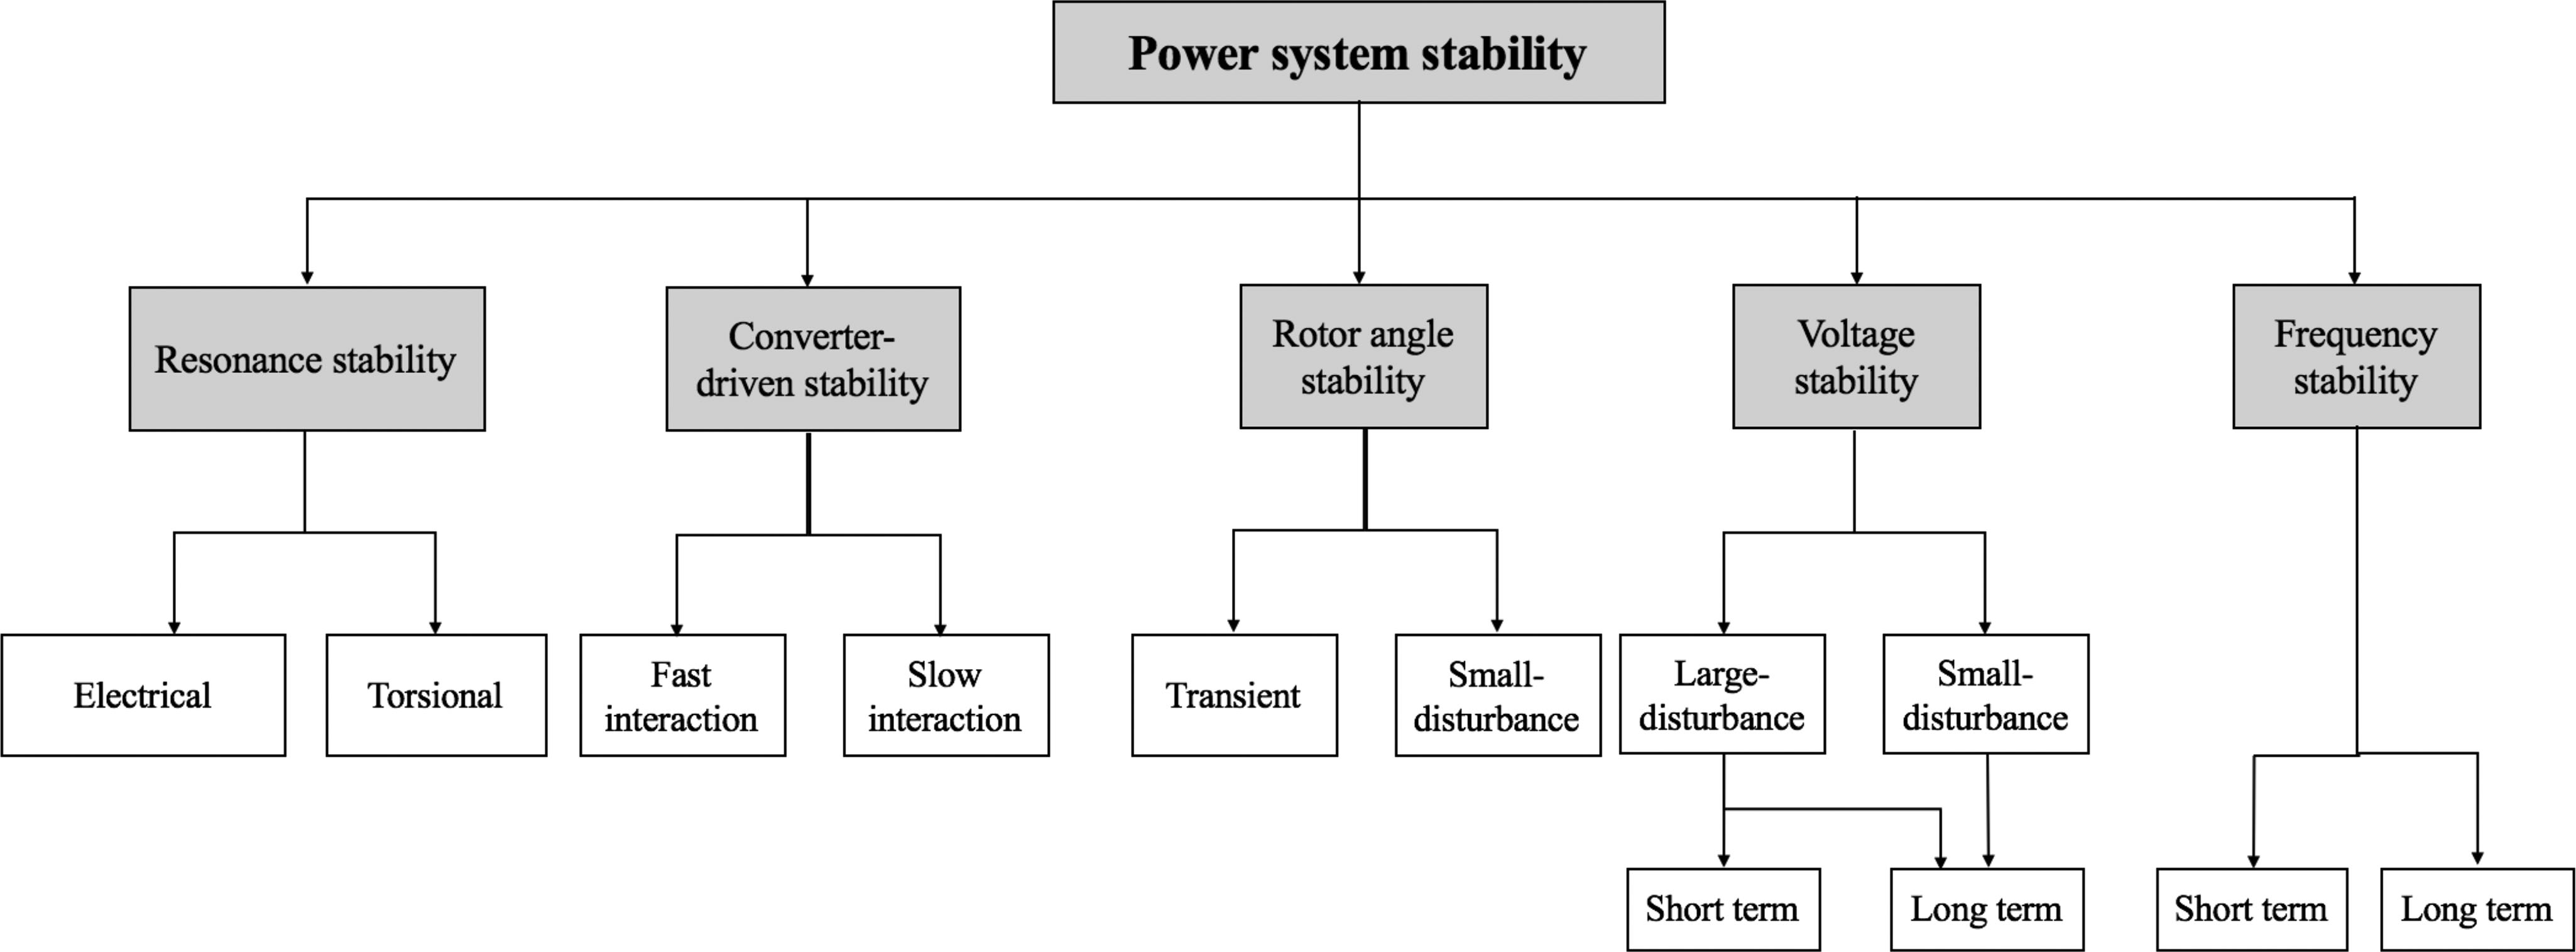
\includegraphics[width=\textwidth]{contents/chapter-2/PowerSystemStabilityClassification}
  \caption[Klasifikasi Stabilitas Sistem Tenaga]{Klasifikasi Stabilitas Sistem Tenaga
  \cite{Definition_and_Classification_of_Power_System_Stability__Revisited_amp_Extended}}
  \label{fig:power_system_stability_classification}
\end{figure}

Stabilitas sistem tenaga diklasifikasikan menjadi lima kategori utama
\cite{Definition_and_Classification_of_Power_System_Stability__Revisited_amp_Extended}:

\begin{enumerate}
  \item \textbf{Stabilitas resonansi} (\textit{resonance stability}): kemampuan sistem
    menghindari eksitasi resonansi yang tidak teredam pada komponen jaringan. Terbagi
    menjadi resonansi \textit{electrical}, yang terjadi antara kapasitansi saluran dan
    induktansi generator, serta resonansi \textit{torsional}, yang melibatkan interaksi
    antara sistem massa-pegas mekanik turbin-generator dan jaringan listrik.
  \item \textbf{Stabilitas berbasis konverter} (\textit{converter-driven stability}):
    kemampuan sistem mempertahankan operasi stabil terhadap interaksi antara kontroler
    konverter dengan komponen jaringan maupun unit pembangkit lainnya. Terbagi menjadi
    interaksi \textit{fast} pada bandwidth kontroler arus konverter tinggi (orde
    milidetik) dan interaksi \textit{slow} yang melibatkan loop kontrol tegangan dan
    daya konverter (orde puluhan milidetik hingga detik). Kategori ini ditambahkan
    untuk mengakomodasi fenomena ketidakstabilan yang muncul akibat dominasi IBR pada
    sistem tenaga modern.
  \item \textbf{Stabilitas sudut rotor} (\textit{rotor angle stability}): kemampuan
    mesin sinkron yang saling terhubung untuk mempertahankan sinkronisasi setelah
    gangguan. Terbagi menjadi \textit{transient stability} untuk gangguan besar dan
    \textit{small-disturbance stability} untuk gangguan kecil, yang menjadi fokus
    penelitian ini.
  \item \textbf{Stabilitas tegangan} (\textit{voltage stability}): kemampuan sistem
    mempertahankan tegangan yang dapat diterima pada seluruh bus setelah gangguan.
    Terbagi berdasarkan besarnya gangguan (\textit{large-disturbance} dan
    \textit{small-disturbance}) serta rentang waktu (\textit{short term} dan
    \textit{long term}).
  \item \textbf{Stabilitas frekuensi} (\textit{frequency stability}): kemampuan sistem
    mempertahankan frekuensi nominal setelah ketidakseimbangan antara pembangkitan dan
    beban. Terbagi menjadi rentang \textit{short term} (regulasi primer, orde detik)
    dan \textit{long term} (regulasi sekunder, orde menit).
\end{enumerate}

Kelima kategori stabilitas tidak sepenuhnya independen. Gangguan besar yang memicu
ketidakstabilan sudut rotor menyebabkan pula deviasi tegangan dan frekuensi yang
signifikan. Kategorisasi ini memudahkan pemilihan model dan metode analisis yang sesuai
dengan fenomena dominan pada setiap rentang waktu \cite{kundur1994power}.

Integrasi PLTB skala besar mengubah karakteristik stabilitas sistem tenaga. Generator
sinkron konvensional menyumbang inersia rotasional dan torsi sinkronisasi alami melalui
kopling elektromagnetik langsung dengan jaringan; turbin angin berbasis konverter
menggantikan sebagian kapasitas tersebut dengan unit pembangkit yang keluarannya
dikontrol secara elektronik. Perubahan komposisi pembangkitan ini memengaruhi kelima
kategori stabilitas, dengan dampak paling terukur pada \textit{small signal stability}
melalui perubahan karakteristik \textit{electromechanical oscillation mode}
\cite{kundur1994power}.

\subsection{Stabilitas Sinyal Kecil}

\textit{Small signal stability} (SSS) adalah kemampuan sistem tenaga untuk mempertahankan
sinkronisasi setelah mengalami gangguan kecil \cite{kundur1994power}. Gangguan diasumsikan
cukup kecil sehingga persamaan diferensial nonlinear sistem dapat dilinearisasi dengan
akurasi yang dapat diterima di sekitar titik operasi. Rentang waktu yang relevan adalah
10--20 detik, yang mencakup dinamika \textit{electromechanical oscillation}.

Kestabilan dalam konteks SSS ditentukan oleh dua komponen torsi pada mesin sinkron
\cite{kundur1994power}:
\begin{itemize}
  \item \textbf{Torsi sinkronisasi} (\textit{synchronizing torque}): komponen torsi yang
    sefasa dengan deviasi sudut rotor $\Delta\delta$. Defisiensi komponen ini menyebabkan
    peningkatan monoton sudut rotor.
  \item \textbf{Torsi redaman} (\textit{damping torque}): komponen torsi yang sefasa
    dengan deviasi kecepatan rotor $\Delta\omega$. Defisiensi komponen ini menyebabkan
    osilasi rotor dengan amplitudo yang terus meningkat.
\end{itemize}

\textit{Electromechanical oscillation mode} terbagi menjadi dua jenis \cite{kundur1994power}:
\begin{itemize}
  \item \textbf{\textit{Local mode}}: osilasi antara satu generator dan sisa sistem,
    pada frekuensi 0{,}8--2{,}0~Hz. Mode ini muncul pada generator yang terhubung
    secara elektrik kuat dalam satu area.
  \item \textbf{\textit{Inter-area mode}}: osilasi antara kelompok generator di satu
    area dan kelompok generator di area lain, pada frekuensi 0{,}1--0{,}8~Hz.
    Saluran transmisi yang lemah antar area menjadi faktor penentu utama.
\end{itemize}

Kriteria redaman yang umum digunakan adalah \textit{damping ratio} $\zeta \geq 5\%$
untuk setiap \textit{electromechanical oscillation mode} \cite{kundur1994power}.

Instabilitas SSS terjadi melalui dua mekanisme \cite{kundur1994power}. Mekanisme
pertama adalah defisiensi torsi sinkronisasi, yang menghasilkan \textit{eigenvalue}
riil positif dan divergensi monoton sudut rotor tanpa komponen osilasi. Mekanisme
kedua adalah defisiensi torsi redaman, yang menghasilkan \textit{eigenvalue} kompleks
dengan bagian riil positif dan osilasi rotor beramplitudo tumbuh. Mekanisme kedua
lebih umum dijumpai pada sistem tenaga modern dan menjadi fokus analisis SSS.

Sistem eksitasi otomatis (AVR) berkecepatan tinggi meningkatkan torsi sinkronisasi
namun dapat mengurangi torsi redaman \cite{kundur1994power}. \textit{Power system
stabilizer} (PSS) dipasang bersama AVR untuk memulihkan torsi redaman yang memadai
melalui sinyal penstabil pada loop eksitasi. Dalam penelitian ini, PSS tidak
dimodelkan agar dampak murni penggantian generator sinkron dengan turbin angin
terhadap redaman alamiah sistem dapat diamati.

\subsection{Persamaan Ayunan}

Persamaan ayunan (\textit{swing equation}) mengatur dinamika rotasi mesin sinkron
\cite{sauer2006power}. Persamaan dasar dalam satuan SI:

\begin{equation}
  J\frac{d^2\theta_m}{dt^2} = T_m - T_e
  \label{eq:swing-basic}
\end{equation}

dengan $J$ adalah momen inersia rotor (kg$\cdot$m$^2$), $\theta_m$ adalah posisi sudut
rotor terhadap sumbu diam (rad mekanis), $T_m$ adalah torsi mekanik, dan $T_e$ adalah
torsi elektromagnetik (N$\cdot$m).

Derivasi ke satuan per unit dimulai dengan menguraikan posisi rotor menjadi komponen
referensi sinkron yang berputar pada $\omega_{sm}$ dan deviasi sudut mekanis $\delta_m$
\cite{kundur1994power}:

\begin{equation}
  \theta_m = \omega_{sm}\,t + \delta_m, \qquad
  \frac{d\theta_m}{dt} = \omega_{sm} + \frac{d\delta_m}{dt}
  \label{eq:swing-decomp}
\end{equation}

sehingga $d^2\theta_m/dt^2 = d^2\delta_m/dt^2$. Perkalian persamaan~\eqref{eq:swing-basic}
dengan kecepatan sudut sesaat $\omega_m$ mengonversi domain torsi ke domain daya
($P_m = T_m\omega_m$, $P_e = T_e\omega_m$):

\begin{equation}
  J\omega_m\,\frac{d^2\delta_m}{dt^2} = P_m - P_e
  \label{eq:swing-power}
\end{equation}

Untuk gangguan kecil $\omega_m \approx \omega_{sm}$, sehingga momentum sudut
$M = J\omega_{sm}$ (kg$\cdot$m$^2$/s) bersifat konstan. Dari definisi konstanta inersia
$H = \tfrac{1}{2}J\omega_{sm}^2 / S_{\text{rated}}$ diperoleh $M = 2H\,S_{\text{rated}}/\omega_{sm}$.
Untuk mesin dengan $P$ kutub, sudut elektris $\delta = (P/2)\,\delta_m$ dan kecepatan
sinkron elektris $\omega_s = (P/2)\,\omega_{sm}$. Setelah normalisasi dengan
$S_{\text{rated}}$, persamaan ayunan dalam satuan per unit menggunakan konstanta inersia
$H$~(MWs/MVA) terurai menjadi dua persamaan diferensial orde pertama yang membentuk
pasangan variabel keadaan $(\omega,\,\delta)$ \cite{sauer2006power}:

\begin{equation}
  \frac{2H}{\omega_s}\frac{d\omega}{dt} = P_m - P_e - D(\omega - \omega_s)
  \label{eq:swing-pu}
\end{equation}

\begin{equation}
  \frac{d\delta}{dt} = \omega - \omega_s
  \label{eq:swing-delta}
\end{equation}

dengan $\omega$ adalah kecepatan sudut rotor, $\delta$ adalah sudut rotor, $P_m$ adalah
daya mekanik masukan, $P_e$ adalah daya elektrik keluaran, dan $D$ adalah koefisien
redaman, semua dalam satuan per unit.

Konstanta inersia $H$ merepresentasikan rasio energi kinetik rotor pada kecepatan
sinkron terhadap daya terkalibrasi mesin \cite{sauer2006power}:

\begin{equation}
  H = \frac{\tfrac{1}{2}J\omega_s^2}{S_{\text{rated}}}
  \label{eq:H-def}
\end{equation}

Nilai $H$ tipikal untuk generator turbin uap berkisar 2--9~MWs/MVA, sedangkan
generator turbin hidro umumnya berada pada rentang 2--4~MWs/MVA \cite{kundur1994power}.
Semakin besar $H$, semakin lambat kecepatan rotor merespons ketidakseimbangan daya,
sehingga frekuensi \textit{electromechanical oscillation} mode tersebut cenderung lebih rendah.

Koefisien redaman $D$ memodelkan efek redaman total yang bekerja pada rotor, mencakup
redaman mekanik bantalan dan efek redaman elektrik \textit{damper winding}. Nilai $D$
yang lebih besar menghasilkan $\sigma_i$ lebih negatif sehingga redaman
\textit{oscillation mode} meningkat \cite{kundur1994power}.

Linearisasi persamaan~\eqref{eq:swing-pu} dan~\eqref{eq:swing-delta} di sekitar titik
operasi $(\delta^0, \omega_s)$ memberikan bentuk matriks yang menghubungkan parameter
fisik langsung ke struktur modal. Mendefinisikan koefisien daya sinkronisasi
$K_s = \partial P_e/\partial\delta\big|_{\delta^0}$ (pu/rad) \cite{kundur1994power}:

\begin{equation}
  \begin{bmatrix}\Delta\dot{\delta} \\[4pt] \Delta\dot{\omega}\end{bmatrix}
  = \underbrace{\begin{bmatrix}
      0 & 1 \\[6pt]
      -\dfrac{\omega_s K_s}{2H} & -\dfrac{\omega_s D}{2H}
    \end{bmatrix}}_{\mathbf{A}_{em}}
  \begin{bmatrix}\Delta\delta \\[4pt] \Delta\omega\end{bmatrix}
  \label{eq:swing-matrix}
\end{equation}

\textit{Eigenvalue} konjugat kompleks matriks $\mathbf{A}_{em}$ adalah:

\begin{equation}
  \lambda = -\frac{\omega_s D}{4H}
    \pm j\sqrt{\frac{\omega_s K_s}{2H} - \left(\frac{\omega_s D}{4H}\right)^2}
  \label{eq:swing-eigenvalue}
\end{equation}

Frekuensi osilasi teredam $\omega_d \approx \sqrt{\omega_s K_s/(2H)}$ (untuk $D$ kecil)
meningkat bersama $K_s$ dan menurun bersama $H$. Bagian riil $\sigma = -\omega_s D/(4H)$
menunjukkan redaman berbanding terbalik dengan $H$: pengurangan $H$ efektif sistem
akibat penetrasi PLTB meningkatkan laju peluruhan modal tetapi sekaligus menggeser
frekuensi \textit{electromechanical oscillation mode} dan memperbesar sensitivitas
sistem terhadap perubahan titik operasi \cite{kundur1994power}.

\subsection{Representasi \textit{State Space}}

Perilaku dinamis sistem tenaga dinyatakan sebagai sistem persamaan
diferensial-aljabar (\textit{differential-algebraic equations}, DAE) nonlinear
\cite{sauer2006power}:

\begin{equation}
  \dot{\mathbf{x}} = \mathbf{f}(\mathbf{x}, \mathbf{u})
  \label{eq:ss-nonlinear}
\end{equation}

\begin{equation}
  \mathbf{y} = \mathbf{g}(\mathbf{x}, \mathbf{u})
  \label{eq:output-nonlinear}
\end{equation}

dengan $\mathbf{x} \in \mathbb{R}^n$ adalah vektor variabel keadaan yang mencakup
seluruh derajat kebebasan dinamik sistem, $\mathbf{u} \in \mathbb{R}^r$ adalah vektor
input, dan $\mathbf{y} \in \mathbb{R}^m$ adalah vektor output sistem. Untuk sistem
IEEE \textit{nine-bus} dengan $n_g$ generator sinkron, vektor keadaan gabungan memiliki
struktur blok:

\begin{equation}
  \mathbf{x} =
  \begin{bmatrix}
    \mathbf{x}_{sg,1}^\top & \mathbf{x}_{sg,2}^\top & \cdots &
    \mathbf{x}_{sg,n_g}^\top & \mathbf{x}_{WT}^\top
  \end{bmatrix}^\top
  \label{eq:state-full}
\end{equation}

dengan $\mathbf{x}_{sg,i} = [\delta_i,\,\omega_i,\,E'_{qi},\,E'_{di}]^\top$ untuk
generator sinkron ke-$i$ dan $\mathbf{x}_{WT}$ untuk variabel keadaan turbin angin
yang menggantikan salah satu generator.

\subsection{Linearisasi}

Untuk analisis SSS, sistem dilinearisasi di sekitar titik ekuilibrium
$(\mathbf{x}_0, \mathbf{u}_0)$ melalui ekspansi deret Taylor orde pertama. Suku
orde dua dan lebih tinggi diabaikan karena gangguan diasumsikan kecil, sehingga
diperoleh sistem linear \cite{kundur1994power}:

\begin{equation}
  \Delta\dot{\mathbf{x}} = \mathbf{A}\,\Delta\mathbf{x} + \mathbf{B}\,\Delta\mathbf{u}
  \label{eq:linear-state}
\end{equation}

\begin{equation}
  \Delta\mathbf{y} = \mathbf{C}\,\Delta\mathbf{x} + \mathbf{D}\,\Delta\mathbf{u}
  \label{eq:linear-output}
\end{equation}

Representasi persamaan~\eqref{eq:linear-state} dan~\eqref{eq:linear-output} dalam
bentuk diagram blok ditunjukkan pada Gambar~\ref{fig:ss_block_diagram}.

\begin{figure}[H]
  \centering
  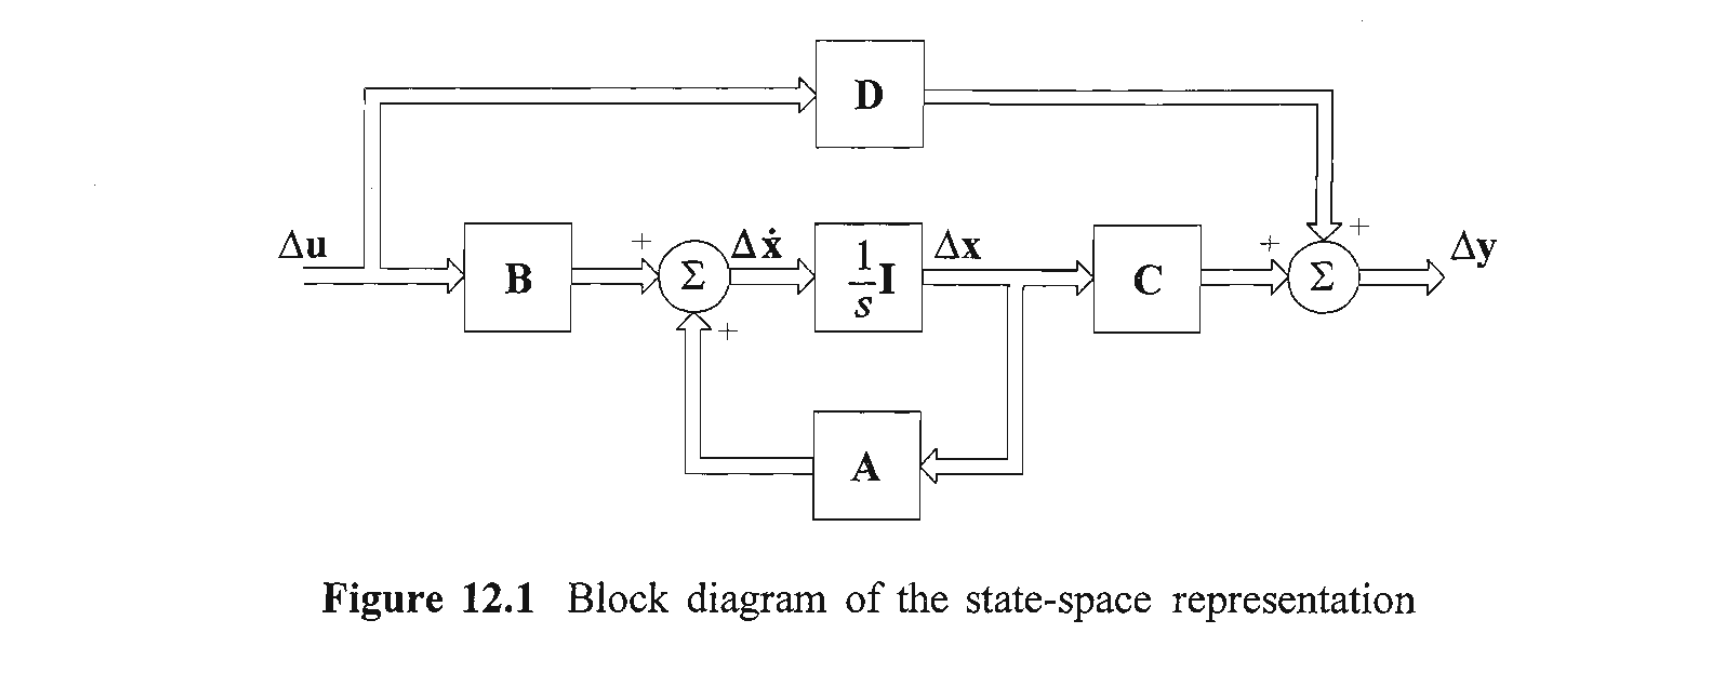
\includegraphics[width=0.80\textwidth]{contents/chapter-2/StateSpaceBlockDiagram}
  \caption[\textit{Block Diagram} Representasi \textit{State Space}]{\textit{Block
  Diagram} Representasi \textit{State Space} \cite{kundur1994power}}
  \label{fig:ss_block_diagram}
\end{figure}

Sinyal $\Delta\mathbf{u}$ masuk melalui blok $\mathbf{B}$ ke penjumlah ($\Sigma$)
yang menghasilkan laju perubahan keadaan $\Delta\dot{\mathbf{x}}$. Integrator
$\tfrac{1}{s}\mathbf{I}$ mengintegrasikan $\Delta\dot{\mathbf{x}}$ menjadi vektor
keadaan $\Delta\mathbf{x}$. Keluaran $\Delta\mathbf{x}$ umpan balik melalui blok
$\mathbf{A}$ ke penjumlah, membentuk loop dinamik sistem. Secara bersamaan,
$\Delta\mathbf{x}$ diteruskan ke blok $\mathbf{C}$ dan $\Delta\mathbf{u}$
diteruskan langsung melalui blok $\mathbf{D}$ (\textit{feedthrough}), keduanya
dijumlahkan di keluaran untuk membentuk $\Delta\mathbf{y}$.

Matriks $\mathbf{A} \in \mathbb{R}^{n \times n}$ adalah matriks sistem (\textit{state
matrix}), dengan elemen $A_{ij} = \partial f_i / \partial x_j$ yang dievaluasi pada
titik ekuilibrium \cite{kundur1994power}:

\begin{equation}
  \mathbf{A} =
  \begin{bmatrix}
    \dfrac{\partial f_1}{\partial x_1} & \dfrac{\partial f_1}{\partial x_2} & \cdots & \dfrac{\partial f_1}{\partial x_n} \\[10pt]
    \dfrac{\partial f_2}{\partial x_1} & \dfrac{\partial f_2}{\partial x_2} & \cdots & \dfrac{\partial f_2}{\partial x_n} \\[6pt]
    \vdots & \vdots & \ddots & \vdots \\[4pt]
    \dfrac{\partial f_n}{\partial x_1} & \dfrac{\partial f_n}{\partial x_2} & \cdots & \dfrac{\partial f_n}{\partial x_n}
  \end{bmatrix}_{\mathbf{x}_0,\,\mathbf{u}_0}
  \label{eq:A-jacobian}
\end{equation}

Matriks $\mathbf{B}$ ($n \times r$), $\mathbf{C}$ ($m \times n$), dan $\mathbf{D}$
($m \times r$) adalah matriks input, output, dan transmisi langsung. Perilaku dinamis
sistem linear ditentukan oleh akar persamaan karakteristik:

\begin{equation}
  \det(s\mathbf{I} - \mathbf{A}) = 0
  \label{eq:char-eq}
\end{equation}

Titik ekuilibrium $(\mathbf{x}_0, \mathbf{u}_0)$ diperoleh dari solusi \textit{load
flow} yang menentukan tegangan bus, sudut tegangan, dan aliran daya dalam kondisi
tunak \cite{sauer2006power}. Nilai-nilai ini digunakan untuk mengevaluasi setiap elemen
$A_{ij} = \partial f_i / \partial x_j$ pada titik operasi.

Orde $n$ matriks $\mathbf{A}$ setara dengan jumlah total variabel keadaan seluruh
komponen dinamik sistem. Untuk sistem dengan $n_g$ generator sinkron model dua sumbu
ditambah kontroler eksitasi, governor, dan turbin angin, orde $n$ dapat mencapai
puluhan hingga ratusan. Setiap \textit{eigenvalue} dari matriks $\mathbf{A}$
merepresentasikan satu mode dinamik sistem; \textit{electromechanical oscillation mode}
adalah subset yang paling relevan untuk penilaian SSS \cite{kundur1994power}.

DIgSILENT PowerFactory 2024 membentuk matriks $\mathbf{A}$ dan menyelesaikan
persamaan~\eqref{eq:char-eq} melalui modul \textit{modal analysis}
pada titik operasi hasil \textit{load flow}.

\subsection{Analisis Stabilitas}

Analisis stabilitas sistem linear dilaksanakan melalui dekomposisi modal matriks
$\mathbf{A}$. Jika $\mathbf{A}$ memiliki $n$ \textit{eigenvalue} yang berbeda, maka
$\mathbf{A}$ dapat difaktorisasi sebagai \cite{kundur1994power}:

\begin{equation}
  \mathbf{A} = \boldsymbol{\Phi}\,\boldsymbol{\Lambda}\,\boldsymbol{\Psi}
  \label{eq:eigendecomp}
\end{equation}

dengan $\boldsymbol{\Lambda} = \mathrm{diag}(\lambda_1, \lambda_2, \ldots, \lambda_n)$
adalah matriks diagonal \textit{eigenvalue}, $\boldsymbol{\Phi} = [\boldsymbol{\phi}_1
\mid \boldsymbol{\phi}_2 \mid \cdots \mid \boldsymbol{\phi}_n]$ adalah matriks
\textit{right eigenvector} (kolom ke-$i$ adalah $\boldsymbol{\phi}_i$), dan
$\boldsymbol{\Psi} = \boldsymbol{\Phi}^{-1}$ adalah matriks \textit{left eigenvector}
(baris ke-$i$ adalah $\boldsymbol{\psi}_i^\top$). Kedua matriks eigenvector memenuhi
kondisi biortogonalitas:

\begin{equation}
  \boldsymbol{\Psi}\,\boldsymbol{\Phi} = \mathbf{I}
  \label{eq:biorthogonal}
\end{equation}

Dengan transformasi modal $\Delta\mathbf{x} = \boldsymbol{\Phi}\,\mathbf{z}$,
persamaan~\eqref{eq:linear-state} (untuk $\Delta\mathbf{u} = \mathbf{0}$) terurai
menjadi $n$ persamaan skalar yang sepenuhnya independen satu sama lain
\cite{sauer2006power}:

\begin{equation}
  \dot{z}_i = \lambda_i\,z_i, \quad z_i(t) = z_i(0)\,e^{\lambda_i t},
  \quad i = 1, 2, \ldots, n
  \label{eq:modal-decoupled}
\end{equation}

sehingga respons bebas $\Delta\mathbf{x}(t)$ merupakan superposisi kontribusi
seluruh mode:

\begin{equation}
  \Delta\mathbf{x}(t) = \sum_{i=1}^{n} c_i\,\boldsymbol{\phi}_i\,e^{\lambda_i t},
  \qquad c_i = \boldsymbol{\psi}_i^\top\,\Delta\mathbf{x}(0)
  \label{eq:free-response}
\end{equation}

\textit{Right eigenvector} $\boldsymbol{\phi}_i$ (\textit{mode shape}) menentukan
distribusi spasial osilasi mode ke-$i$, sedangkan \textit{left eigenvector}
$\boldsymbol{\psi}_i$ menentukan sensitivitas mode ke-$i$ terhadap kondisi awal.
Stabilitas global sistem ditentukan oleh tanda bagian riil setiap \textit{eigenvalue}
$\lambda_i$. DIgSILENT PowerFactory 2024 melaksanakan dekomposisi ini secara numerik
setelah membentuk $\mathbf{A}$ dari titik operasi \textit{load flow}, kemudian
menghitung seluruh \textit{eigenvalue}, \textit{eigenvector}, dan
\textit{participation factor}.

\subsubsection{\textit{Eigenvalue} dan Stabilitas}

Akar persamaan karakteristik~\eqref{eq:char-eq} adalah \textit{eigenvalue} matriks
sistem $\mathbf{A}$. Setiap \textit{electromechanical oscillation mode} bersesuaian
dengan sepasang \textit{eigenvalue} konjugat kompleks \cite{kundur1994power}:

\begin{equation}
  \lambda_i = \sigma_i \pm j\omega_i
  \label{eq:def-eigenvalue}
\end{equation}

Bagian riil $\sigma_i$ menentukan karakteristik redaman: $\sigma_i < 0$ berarti
amplitudo osilasi meluruh secara eksponensial (mode stabil), sedangkan $\sigma_i > 0$
berarti amplitudo tumbuh sehingga mode tidak stabil. \textit{Eigenvalue} real murni
($\omega_i = 0$) bersesuaian dengan mode aperiodik, sedangkan $\omega_i \neq 0$
menghasilkan respons osilatorik. Dalam konteks SSS, sistem dinyatakan tidak stabil
apabila terdapat minimal satu \textit{eigenvalue} dengan $\sigma_i > 0$.

Posisi \textit{eigenvalue} pada bidang kompleks (\textit{eigenvalue plot}) mencerminkan
margin kestabilan: makin negatif $\sigma_i$, makin besar margin redaman mode tersebut.
Pada \textit{electromechanical mode}, \textit{mode shape} $\boldsymbol{\phi}_i$
memperlihatkan amplitudo dan fase relatif osilasi setiap variabel sudut rotor:
generator dengan elemen $\phi_{ki}$ (terkait $\delta_k$) berfasa berlawanan berayun
satu terhadap lainnya, membentuk pola osilasi yang membedakan mode \textit{local}
(0{,}8--2{,}0~Hz) dari mode \textit{inter-area} (0{,}1--0{,}8~Hz) \cite{kundur1994power}.

\subsubsection{\textit{Damping Ratio}}

\textit{Damping ratio} $\zeta_i$ mengkuantifikasi laju peluruhan relatif amplitudo
osilasi terhadap frekuensi osilasi, dihitung dari komponen riil dan imajiner
\textit{eigenvalue} \cite{kundur1994power}:

\begin{equation}
  \zeta_i = \frac{-\sigma_i}{\sqrt{\sigma_i^2 + \omega_i^2}}
  \label{eq:damping-ratio}
\end{equation}

Frekuensi osilasi teredam dalam satuan Hz:

\begin{equation}
  f_i = \frac{\omega_i}{2\pi}
  \label{eq:freq-osc}
\end{equation}

Nilai $\zeta_i$ berada pada rentang $[0,\,1]$ untuk mode osilatorik: $\zeta_i = 0$
bersesuaian dengan osilasi tanpa redaman ($\sigma_i = 0$, batas kestabilan),
sedangkan $\zeta_i = 1$ bersesuaian dengan sistem \textit{critically damped}. Standar
kestabilan yang umum diterapkan pada sistem tenaga adalah $\zeta_i \geq 5\%$ untuk
setiap \textit{electromechanical oscillation mode} \cite{kundur1994power}. Mode dengan
$0 < \zeta_i < 5\%$ diklasifikasikan sebagai \textit{poorly damped} dan berpotensi
menimbulkan osilasi berkepanjangan pasca-gangguan yang dapat memicu
\textit{tripping} proteksi.

\subsubsection{\textit{Participation Factor}}

\textit{Participation factor} $P_{ki}$ mengukur derajat keterlibatan variabel keadaan
ke-$k$ dalam \textit{oscillation mode} ke-$i$ \cite{kundur1994power}:

\begin{equation}
  P_{ki} = \phi_{ki}\,\psi_{ik}
  \label{eq:pf}
\end{equation}

dengan $\phi_{ki}$ adalah elemen ke-$k$ dari \textit{right eigenvector} mode ke-$i$,
dan $\psi_{ik}$ adalah elemen ke-$k$ dari \textit{left eigenvector} mode ke-$i$.
Karena merupakan hasil kali pasangan elemen \textit{right} dan \textit{left
eigenvector}, $P_{ki}$ tidak bergantung pada normalisasi maupun satuan variabel
keadaan sehingga bersifat tidak berdimensi. Matriks \textit{participation factor}
$\mathbf{P}$ memiliki properti bahwa jumlah setiap kolom (kontribusi semua variabel
keadaan pada satu mode) bernilai satu \cite{kundur1994power}.

Dalam analisis sistem tenaga multi-mesin, nilai $|P_{ki}|$ pada \textit{electromechanical mode}
biasanya terkonsentrasi pada variabel $\delta_k$ dan $\omega_k$ generator-generator
yang berayun satu terhadap lainnya. Pada sistem dengan penetrasi turbin angin,
distribusi $|P_{ki}|$ juga mengungkap keterlibatan variabel keadaan kontroler
konverter (integrator RSC/GSC, keadaan PLL) dalam \textit{electromechanical mode};
informasi ini tidak diperoleh dari \textit{eigenvalue} dan \textit{damping ratio}
saja \cite{kundur1994power}. Informasi ini digunakan untuk menilai pergeseran
keterlibatan variabel keadaan akibat penggantian generator sinkron dengan turbin
angin berbasis konverter.

\subsection{Generator Sinkron}

Generator sinkron dimodelkan dengan model dua sumbu (\textit{two-axis model}) yang
memperhitungkan dinamika fluks transien pada sumbu $d$ dan $q$ \cite{sauer2006power}.
Model ini memiliki empat variabel keadaan per mesin yang tersusun dalam vektor:

\begin{equation}
  \mathbf{x}_{sg} = \begin{bmatrix}\delta & \omega & E'_q & E'_d\end{bmatrix}^\top
  \label{eq:sg-statevec}
\end{equation}

dengan $\delta$ adalah sudut rotor, $\omega$ adalah kecepatan sudut, $E'_q$ adalah
tegangan transien sumbu $q$, dan $E'_d$ adalah tegangan transien sumbu $d$.
Persamaan dinamik keempat variabel keadaan dalam satuan per unit \cite{sauer2006power}
dirangkum dalam bentuk vektor:

\begin{equation}
  \frac{d\mathbf{x}_{sg}}{dt} =
  \begin{bmatrix}
    \omega - \omega_s \\[6pt]
    \dfrac{\omega_s}{2H}\bigl[T_m - T_e - D(\omega - \omega_s)\bigr] \\[8pt]
    \dfrac{1}{T'_{do}}\bigl[E_{fd} - E'_q - (x_d - x'_d)\,I_d\bigr] \\[8pt]
    \dfrac{1}{T'_{qo}}\bigl[-E'_d + (x_q - x'_q)\,I_q\bigr]
  \end{bmatrix}
  \label{eq:sg-vector}
\end{equation}

Persamaan dinamik mesin secara individual dalam satuan per unit \cite{sauer2006power}:

\begin{align}
  \frac{d\delta}{dt} &= \omega - \omega_s
  \label{eq:sg-delta} \\[4pt]
  \frac{2H}{\omega_s}\frac{d\omega}{dt} &= T_m - T_e - D(\omega - \omega_s)
  \label{eq:sg-omega} \\[4pt]
  T'_{do}\frac{dE'_q}{dt} &= E_{fd} - E'_q - (x_d - x'_d)\,I_d
  \label{eq:sg-Eq} \\[4pt]
  T'_{qo}\frac{dE'_d}{dt} &= -E'_d + (x_q - x'_q)\,I_q
  \label{eq:sg-Ed}
\end{align}

dengan $T'_{do}$ dan $T'_{qo}$ adalah konstanta waktu transien lingkar terbuka sumbu
$d$ dan $q$, $x_d$ dan $x_q$ adalah reaktansi sinkron, $x'_d$ dan $x'_q$ adalah
reaktansi transien, dan $E_{fd}$ adalah tegangan medan (keluaran sistem eksitasi).

Persamaan aljabar stator menghubungkan tegangan terminal dengan arus:

\begin{align}
  V_d &= -R_a I_d + x'_q I_q + E'_d
  \label{eq:sg-Vd} \\[4pt]
  V_q &= -R_a I_q - x'_d I_d + E'_q
  \label{eq:sg-Vq}
\end{align}

dengan $R_a$ adalah resistansi jangkar, $I_d$ dan $I_q$ adalah arus sumbu $d$ dan
$q$, serta $V_d$ dan $V_q$ adalah tegangan terminal sumbu $d$ dan $q$. Torsi
elektromagnetik dihitung sebagai:

\begin{equation}
  T_e = E'_q I_q + E'_d I_d + (x'_d - x'_q)\,I_d I_q
  \label{eq:sg-Te}
\end{equation}

Model dua sumbu dipilih karena mempertahankan dinamika fluks transien sumbu $d$ dan
$q$ yang relevan untuk SSS pada rentang waktu 10--20 detik \cite{sauer2006power}.
Model klasik yang hanya menyertakan variabel $(\delta, \omega)$ tidak memadai karena
mengabaikan pengaruh sistem eksitasi pada redaman osilasi. Variabel $E'_q$ dan $E'_d$
merepresentasikan tegangan internal transien yang terkait langsung dengan fluks di
masing-masing sumbu; keduanya dipengaruhi oleh tegangan medan $E_{fd}$ yang merupakan
keluaran AVR. Dinamika AVR ditambahkan sebagai subsistem terpisah dalam \textit{template}
DIgSILENT PowerFactory 2024 dan digabungkan ke dalam matriks $\mathbf{A}$ secara
keseluruhan.

Dalam penelitian ini, ketiga generator sinkron pada sistem IEEE \textit{nine-bus}
dimodelkan menggunakan model dua sumbu bawaan DIgSILENT PowerFactory 2024.
Persamaan~\eqref{eq:sg-delta}--\eqref{eq:sg-Te} terbentuk sebagai bagian dari
matriks $\mathbf{A}$ sistem.

\subsubsection{Model PowerFactory: Variabel Fluks Subtransien}

Model standar DIgSILENT PowerFactory 2024 mengimplementasikan mesin sinkron
menggunakan fluks rotor sebagai variabel keadaan, berbeda dari model dua sumbu
klasik yang menggunakan tegangan transien $E'_q$ dan $E'_d$. Model ini mengacu
pada representasi rangkaian ekivalen orde kedua dalam koordinat referensi rotor
(\textit{Park coordinates}) \cite{digsilent2024sm}. Sumbu $d$ selalu dimodelkan
dengan dua loop rotor: belitan medan (\textit{field winding}, fd) dan
\textit{damper winding} 1d. Sumbu $q$ mendukung dua varian: model \textit{salient-pole}
dengan satu \textit{damper winding} 1q (Model 2.1) dan model \textit{round-rotor}
dengan dua \textit{damper winding} 1q dan 2q (Model 2.2) sesuai panduan IEEE
\cite{digsilent2024sm}. Rangkaian ekivalen sumbu $d$ dan sumbu $q$ model
PowerFactory ditunjukkan pada Gambar~\ref{fig:sg_pf_daxis} dan
Gambar~\ref{fig:sg_pf_qaxis}.

\begin{figure}[H]
  \centering
  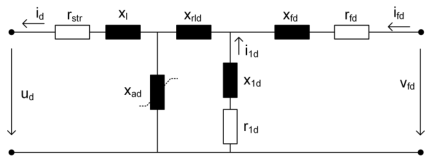
\includegraphics[width=0.85\textwidth]{contents/chapter-2/SG_daxis}
  \caption[\textit{D-Axis Equivalent Circuit} Generator Sinkron PowerFactory]
  {\textit{D-Axis Equivalent Circuit} Generator Sinkron PowerFactory \cite{digsilent2024sm}}
  \label{fig:sg_pf_daxis}
\end{figure}

\begin{figure}[H]
  \centering
  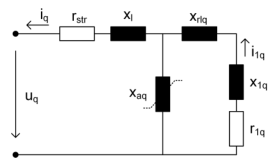
\includegraphics[width=0.70\textwidth]{contents/chapter-2/SG_qaxis}
  \caption[\textit{Q-Axis Equivalent Circuit} Generator Sinkron PowerFactory
  (\textit{Salient-Pole})]{\textit{Q-Axis Equivalent Circuit} Generator Sinkron
  PowerFactory (\textit{Salient-Pole}) \cite{digsilent2024sm}}
  \label{fig:sg_pf_qaxis}
\end{figure}

Persamaan tegangan stator dalam kerangka referensi rotor, dengan $n$ adalah kecepatan
rotor per unit dan $\omega_n = 2\pi f_{nom}$ adalah frekuensi sudut nominal
\cite{digsilent2024sm}:

\begin{align}
  u_d &= -r_{str}\,i_d - n\,\psi_q + \frac{1}{\omega_n}\frac{d\psi_d}{dt}
  \label{eq:sg-pf-ud} \\[4pt]
  u_q &= -r_{str}\,i_q + n\,\psi_d + \frac{1}{\omega_n}\frac{d\psi_q}{dt}
  \label{eq:sg-pf-uq}
\end{align}

Persamaan belitan rotor (medan dan \textit{damper}) mengintegrasikan dinamika fluks
dengan resistansi per loop \cite{digsilent2024sm}:

\begin{equation}
  v_{fd} = r_{fd}\,i_{fd} + \frac{1}{\omega_n}\frac{d\psi_{fd}}{dt}, \quad
  0 = r_{1d}\,i_{1d} + \frac{1}{\omega_n}\frac{d\psi_{1d}}{dt}, \quad
  0 = r_{1q}\,i_{1q} + \frac{1}{\omega_n}\frac{d\psi_{1q}}{dt}
  \label{eq:sg-pf-rotor}
\end{equation}

dengan $v_{fd}$ adalah tegangan belitan medan keluaran AVR dalam satuan per unit, dan
\textit{damper winding} terhubung pendek sehingga persamaannya homogen.

Untuk simulasi stabilitas RMS, suku turunan fluks stator $d\psi_s/dt$ diabaikan karena
konstanta waktu transien stator jauh lebih kecil dari rentang waktu
\textit{electromechanical oscillation} (10--20~s). Setelah penyederhanaan ini,
tegangan subtransien dinyatakan sebagai fungsi langsung fluks subtransien
\cite{digsilent2024sm}:

\begin{equation}
  u''_d = -n\,\psi''_q, \qquad u''_q = n\,\psi''_d
  \label{eq:sg-pf-subtrans}
\end{equation}

dan persamaan tegangan stator menjadi representasi
\textit{voltage-behind-subtransient-reactance}:

\begin{equation}
  u_d = u''_d - r_{str}\,i_d + n\,x''_q\,i_q, \qquad
  u_q = u''_q - r_{str}\,i_q - n\,x''_d\,i_d
  \label{eq:sg-pf-rms-volt}
\end{equation}

Torsi elektrik dihitung dari arus dan fluks stator dengan normalisasi faktor daya
terkalibrasi $cosn$ \cite{digsilent2024sm}:

\begin{equation}
  t_e = \frac{i_q\,\psi_d - i_d\,\psi_q}{cosn}
  \label{eq:sg-pf-te}
\end{equation}

Vektor variabel keadaan model RMS PowerFactory untuk mesin \textit{round-rotor} adalah:

\begin{equation}
  \mathbf{x}_{sg,PF} =
  \begin{bmatrix}\varphi & n & \psi_{fd} & \psi_{1d} & \psi_{1q} & \psi_{2q}\end{bmatrix}^\top
  \label{eq:sg-pf-statevec}
\end{equation}

dengan $\varphi$ adalah posisi sudut rotor dalam elektris radian dan $n$ adalah kecepatan
rotor per unit. Untuk mesin \textit{salient-pole}, $\psi_{2q}$ dihilangkan sehingga
orde model menjadi 5. Keterkaitan model subtransien PowerFactory dengan model dua sumbu
klasik~\eqref{eq:sg-Eq}--\eqref{eq:sg-Ed} terbentuk melalui pemetaan: tegangan transien
$E'_q$ bersesuaian dengan komponen fluks subtransien sumbu $q$, dan $E'_d$ bersesuaian
dengan komponen sumbu $d$; keduanya menghasilkan matriks sistem $\mathbf{A}$ yang
ekivalen untuk analisis SSS \cite{digsilent2024sm}.

Parameter masukan model standar PowerFactory ditabulasikan pada
Tabel~\ref{tab:sg-pf-params}.

\begin{table}[H]
\centering
\caption[Parameter Masukan Model Standar Generator Sinkron DIgSILENT PowerFactory 2024]{Parameter Masukan Model Standar Generator Sinkron DIgSILENT PowerFactory 2024
\cite{digsilent2024sm}}
\label{tab:sg-pf-params}
\small
\begin{tabular}{p{1.8cm} p{1.4cm} p{0.9cm} p{8.1cm}}
\toprule
\textbf{Param. PF} & \textbf{Simbol} & \textbf{Sat.} & \textbf{Deskripsi} \\
\midrule
\texttt{rstr} & $r_{str}$ & p.u. & Resistansi stator \\
\texttt{xl}   & $x_l$    & p.u. & Reaktansi bocor stator \\
\texttt{xad}  & $x_{ad}$ & p.u. & Reaktansi magnetisasi sumbu $d$ \\
\texttt{xaq}  & $x_{aq}$ & p.u. & Reaktansi magnetisasi sumbu $q$ \\
\texttt{xfd}  & $x_{fd}$ & p.u. & Reaktansi belitan medan (sumbu $d$) \\
\texttt{x1d}  & $x_{1d}$ & p.u. & Reaktansi \textit{damper winding} 1d \\
\texttt{x1q}  & $x_{1q}$ & p.u. & Reaktansi \textit{damper winding} 1q \\
\texttt{x2q}  & $x_{2q}$ & p.u. & Reaktansi \textit{damper winding} 2q \\
\texttt{rfd}  & $r_{fd}$ & p.u. & Resistansi belitan medan \\
\texttt{r1d}  & $r_{1d}$ & p.u. & Resistansi \textit{damper winding} 1d \\
\texttt{r1q}  & $r_{1q}$ & p.u. & Resistansi \textit{damper winding} 1q \\
\texttt{r2q}  & $r_{2q}$ & p.u. & Resistansi \textit{damper winding} 2q \\
\texttt{tds}  & $t'_d$   & s    & Konstanta waktu transien singkat sumbu $d$ \\
\texttt{tdss} & $t''_d$  & s    & Konstanta waktu subtransien singkat sumbu $d$ \\
\bottomrule
\end{tabular}
\end{table}

\subsection{Pemodelan DFIG-WT}

DFIG-WT (\textit{Doubly Fed Induction Generator Wind Turbine}, Tipe 3) merupakan
teknologi turbin angin kecepatan variabel yang paling banyak diinstalasi secara
global karena keunggulan biaya konverternya. Topologi sistem DFIG-WT, sebagaimana
ditunjukkan pada Gambar \ref{fig:dfig_model_ch2}, terdiri dari sudu turbin yang
menggerakkan \textit{gearbox} peningkat putaran, DFIG (generator induksi rotor
belitan), \textit{Rotor-Side Converter} (RSC) sebagai konverter AC/DC terkontrol,
DC Bus dengan kapasitor penyangga, dan \textit{Grid-Side Converter} (GSC) sebagai
inverter DC/AC terkontrol yang titik sambungnya paralel dengan stator pada sisi
jaringan \cite{doublyfedinduction}.

\begin{figure}[H]
  \centering
  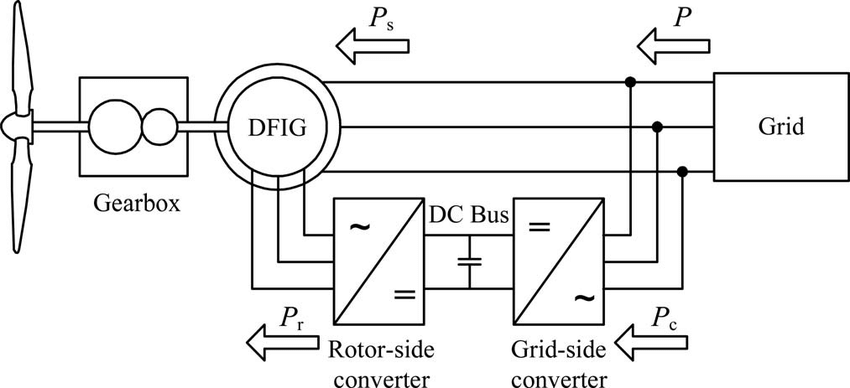
\includegraphics[width=0.85\textwidth]{contents/chapter-2/DFIGModel}
  \caption[Topologi Sistem DFIG-WT]{Topologi Sistem DFIG-WT \cite{doublyfedinduction}}
  \label{fig:dfig_model_ch2}
\end{figure}

Karakteristik fundamental yang membedakan DFIG-WT dari teknologi Tipe 4 adalah
koneksi ganda (\textit{doubly fed}): stator terhubung langsung ke jaringan
menyalurkan daya stator $P_s$, sementara rotor terhubung ke jaringan melalui
rangkaian konverter \textit{back-to-back} RSC--DC Bus--GSC yang menyalurkan daya
rotor $P_r$ dan daya konverter $P_c$. Total daya yang disuntikkan ke jaringan
merupakan superposisi keduanya:

\begin{equation}
  P = P_s + P_c
  \label{eq:dfig-power-total}
\end{equation}

Hubungan antara $P_s$, $P_r$, dan daya mekanik $P_m$ ditentukan oleh slip $s =
(\omega_s - \omega_r)/\omega_s$, yaitu $P_s = (1-s)P_m$ dan $P_r = -sP_m$.
Karena DFIG beroperasi pada rentang slip $s \in [-0{,}3,\; +0{,}3]$, hanya sekitar
25--30\% daya terkalibrasi mengalir melalui konverter, sehingga RSC dan GSC dapat
dirancang dengan kapasitas \textit{partial-rated} yang jauh lebih kecil dan murah
dibandingkan topologi konverter penuh Tipe 4. Pada kondisi \textit{super-synchronous}
($s < 0$), $P_r$ bernilai negatif sehingga daya mengalir dari rotor ke jaringan
melalui GSC; pada kondisi \textit{sub-synchronous} ($s > 0$), daya mengalir
sebaliknya dari jaringan ke rotor melalui GSC dan RSC.

Karena stator terhubung langsung ke jaringan, \textit{flux linkage} $\Psi_{ds}$
dan $\Psi_{qs}$ terkopel dengan tegangan jaringan; variabel keadaan ini berpartisipasi
dalam \textit{electromechanical oscillation mode} sistem. Pada PMSG-WT, konverter
penuh mengisolasi seluruh variabel keadaan generator dari jaringan \cite{knuppel2009small}.

Dinamika listrik DFIG dimodelkan dalam kerangka referensi sinkron yang berputar dengan
kecepatan sudut jaringan $\omega_s$. Persamaan \textit{flux linkage} stator dan rotor
memiliki bentuk simetris dengan perbedaan pada suku frekuensi slip yang muncul pada
persamaan rotor \cite{mehta2014}:

\begin{align}
  \frac{1}{\omega_s}\frac{d\Psi_{qs}}{dt} &= V_{qs} + R_s I_{qs} - \Psi_{ds}
  \label{eq:dfig-psiqs} \\[4pt]
  \frac{1}{\omega_s}\frac{d\Psi_{ds}}{dt} &= V_{ds} + R_s I_{ds} + \Psi_{qs}
  \label{eq:dfig-psids} \\[4pt]
  \frac{1}{\omega_s}\frac{d\Psi_{qr}}{dt} &= V_{qr} - R_r I_{qr}
    - \frac{\omega_s - \omega_r}{\omega_s}\Psi_{dr}
  \label{eq:dfig-psiqr} \\[4pt]
  \frac{1}{\omega_s}\frac{d\Psi_{dr}}{dt} &= V_{dr} - R_r I_{dr}
    + \frac{\omega_s - \omega_r}{\omega_s}\Psi_{qr}
  \label{eq:dfig-psidr}
\end{align}

dengan subskrip $s$ untuk stator dan $r$ untuk rotor; $\Psi$, $V$, $I$, dan $R$
masing-masing adalah \textit{flux linkage}, tegangan, arus, dan resistansi pada
sumbu $q$ atau $d$; serta $\omega_r$ adalah kecepatan sudut rotor. Suku
$\frac{\omega_s - \omega_r}{\omega_s}\Psi_{dr}$ dan
$\frac{\omega_s - \omega_r}{\omega_s}\Psi_{qr}$ pada persamaan rotor merupakan
gaya gerak listrik (\textit{back-EMF}) slip yang besarnya proporsional terhadap
deviasi kecepatan rotor dari kecepatan sinkron. Suku inilah yang menciptakan
kopling dinamik antara variabel keadaan rotor dan kecepatan $\omega_r$, menjadikan
DFIG-WT memiliki interaksi modal yang lebih kompleks dengan sistem jaringan
dibandingkan PMSG-WT.

Hubungan \textit{flux linkage} dengan arus stator dan rotor dinyatakan melalui
induktansi magnetisasi $L_m$, induktansi stator $L_s = L_{ls} + L_m$, dan
induktansi rotor $L_r = L_{lr} + L_m$ \cite{mehta2014}:

\begin{align}
  \Psi_{qs} &= L_s I_{qs} + L_m I_{qr}, \quad
  \Psi_{ds} = L_s I_{ds} + L_m I_{dr} \label{eq:dfig-psi-stator} \\[4pt]
  \Psi_{qr} &= L_r I_{qr} + L_m I_{qs}, \quad
  \Psi_{dr} = L_r I_{dr} + L_m I_{ds} \label{eq:dfig-psi-rotor}
\end{align}

Torsi elektromagnetik yang dibangkitkan DFIG diekspresikan sebagai hasil silang
\textit{flux linkage} dan arus stator dalam kerangka referensi $dq$ \cite{mehta2014}:

\begin{equation}
  T_e = \Psi_{ds} I_{qs} - \Psi_{qs} I_{ds}
  \label{eq:dfig-Te}
\end{equation}

Dinamika mekanik rotor DFIG-WT dinyatakan oleh persamaan ayunan massa tunggal
yang menghubungkan torsi mekanik $T_m$ dari turbin dengan torsi elektromagnetik
$T_e$ \cite{mehta2014}:

\begin{equation}
  \frac{2H_r}{\omega_s}\frac{d\omega_r}{dt} = T_m - T_e
  \label{eq:dfig-omega}
\end{equation}

dengan $H_r$ adalah konstanta inersia rotor DFIG-WT. Variabel keadaan model linearisasi DFIG-WT tersusun dalam vektor:

\begin{equation}
  \mathbf{x}_{DFIG} =
  \begin{bmatrix}\Psi_{qs} & \Psi_{ds} & \Psi_{qr} & \Psi_{dr} & \omega_r\end{bmatrix}^\top
  \label{eq:dfig-statevec}
\end{equation}

di mana $\Psi_{qs}$ dan $\Psi_{ds}$ berpartisipasi langsung dalam
\textit{electromechanical oscillation mode} karena keterkaitan stator dengan tegangan
jaringan, sedangkan $\Psi_{qr}$, $\Psi_{dr}$, dan $\omega_r$ terkopel melalui suku
slip \textit{back-EMF}.

RSC dikendalikan menggunakan strategi orientasi fluks stator (\textit{stator-flux
oriented control}, SFOC), di mana vektor fluks stator dikunci pada sumbu $d$ kerangka
referensi sehingga $\Psi_{qs} = 0$ dan $\Psi_{ds} = |\Psi_s|$. Dalam kondisi ini,
daya aktif stator $P_s \propto I_{qr}$ dan daya reaktif stator $Q_s \propto I_{dr}$,
sehingga RSC controller mengatur $I_{qr}$ untuk pelacakan titik daya maksimum (MPPT)
dan mengatur $I_{dr}$ untuk pengendalian tegangan terminal atau faktor daya
\cite{mehta2014}. GSC mempertahankan tegangan tautan DC $V_{dc}$ pada nilai referensi
dan mengatur pertukaran daya reaktif $P_c$ sisi jaringan secara independen dari RSC,
memberikan DFIG-WT kemampuan pembangkitan daya reaktif dari dua jalur secara simultan.

Dalam penelitian ini, model DFIG-WT menggunakan \textit{template} bawaan DIgSILENT
PowerFactory 2024 \cite{digsilent2024dfig} tanpa modifikasi parameter kontrol.

\subsubsection{Model Elektris Mesin Induksi: Formulasi Matriks Umum}

DFIG diimplementasikan di PowerFactory sebagai mesin induksi asinkron (elemen
\texttt{ElmAsm}) dengan injeksi tegangan rotor aktif. Rangkaian ekivalen mesin
induksi DFIG ditunjukkan pada Gambar~\ref{fig:im_equiv_circuit}.

\begin{figure}[H]
  \centering
  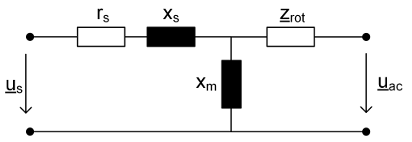
\includegraphics[width=0.75\textwidth]{contents/chapter-2/DFIG_ekivalen}
  \caption[Rangkaian Ekivalen Mesin Induksi (DFIG)]{Rangkaian Ekivalen Mesin
  Induksi (DFIG) \cite{digsilent2024asm}}
  \label{fig:im_equiv_circuit}
\end{figure}

Dinamika listrik mesin induksi dengan $n$ loop rotor dalam kerangka referensi
berputar dengan kecepatan $\omega$ dinyatakan sebagai \cite{digsilent2024asm}:

\begin{equation}
  \underline{u}_S = r_S\,\underline{i}_S + \frac{1}{\omega_n}\frac{d\underline{\Psi}_S}{dt}
    + j\frac{\omega}{\omega_n}\,\underline{\Psi}_S
  \label{eq:im-us}
\end{equation}

\begin{equation}
  \mathbf{0} = \mathbf{r}_R\,\underline{\mathbf{i}}_R
    + \frac{1}{\omega_n}\frac{d\underline{\boldsymbol{\Psi}}_R}{dt}
    + j\frac{\omega - \omega_R}{\omega_n}\,\underline{\boldsymbol{\Psi}}_R
  \label{eq:im-ur-cage}
\end{equation}

dengan $\underline{\boldsymbol{\Psi}}_R$ adalah vektor fluks rotor berdimensi $n$,
$\mathbf{r}_R$ adalah matriks resistansi rotor $n \times n$, dan $\omega_R$ adalah
kecepatan sudut rotor. Persamaan \textit{flux linkage} dalam bentuk matriks
\cite{digsilent2024asm}:

\begin{equation}
  \underline{\Psi}_S = x_{SS}\,\underline{i}_S + \mathbf{x}_{SR}^\top\,\underline{\mathbf{i}}_R,
  \qquad
  \underline{\boldsymbol{\Psi}}_R = \mathbf{x}_{RS}\,\underline{i}_S
    + \mathbf{x}_{RR}\,\underline{\mathbf{i}}_R
  \label{eq:im-flux}
\end{equation}

Untuk model \textit{single cage}, matriks dalam persamaan~\eqref{eq:im-flux} menjadi
skalar: $x_{SS} = x_S + x_m$, $\mathbf{x}_{SR}^\top = x_m$,
$\mathbf{x}_{RR} = x_{rA} + x_m$, dengan $x_m$ adalah reaktansi magnetisasi dan
$x_{rA}$ adalah reaktansi bocor rotor. Untuk model \textit{double cage} (dua loop
rotor), $\mathbf{x}_{RR}$ menjadi matriks $2 \times 2$ yang mencakup reaktansi mutual
antar-sangkar $x_{rm}$ \cite{digsilent2024asm}:

\begin{equation}
  \mathbf{x}_{RR} = \begin{bmatrix}
    x_{rA1} + x_{rA0} + x_m & x_{rA0} + x_m \\
    x_{rA0} + x_m & x_{rA2} + x_{rA0} + x_m
  \end{bmatrix}
  \label{eq:im-xrr-double}
\end{equation}

Reaktansi subtransien diperoleh dari kondensasi Schur matriks impedansi
\cite{digsilent2024asm}:

\begin{equation}
  x'' = x_{SS} - \mathbf{x}_{SR}^\top\,\mathbf{x}_{RR}^{-1}\,\mathbf{x}_{RS}
  \label{eq:im-xpp}
\end{equation}

Untuk simulasi stabilitas RMS, transien stator diabaikan sehingga representasi
\textit{voltage-behind-subtransient-reactance} berlaku \cite{digsilent2024asm}:

\begin{equation}
  \underline{u}_S = r_S\,\underline{i}_S + j\frac{\omega_{ref}}{\omega_n}\,x''\,\underline{i}_S
    + \underline{u}'', \qquad
  \underline{u}'' = j\frac{\omega_{ref}}{\omega_n}\,\underline{\psi}''
  \label{eq:im-rms}
\end{equation}

dengan $\underline{\psi}'' = \mathbf{x}_{SR}^\top\,\mathbf{x}_{RR}^{-1}\,\underline{\boldsymbol{\Psi}}_R$
adalah fluks subtransien yang bergantung hanya pada fluks rotor.

\subsubsection{Persamaan Tegangan Rotor DFIG dan Kerangka Referensi Sinkron}

Untuk DFIG, persamaan rotor~\eqref{eq:im-ur-cage} dimodifikasi dengan memasukkan
tegangan rotor aktif $\underline{u}_{ac}$ yang diinjeksikan RSC, sebagaimana
ditunjukkan pada Gambar~\ref{fig:dfig_equiv_pwm} \cite{digsilent2024doubly}:

\begin{equation}
  \underline{u}_{ac} = r_R\,\underline{i}_R + \frac{1}{\omega_n}\frac{d\underline{\Psi}_R}{dt}
    + j\frac{\omega_{ref} - \omega_R}{\omega_n}\,\underline{\Psi}_R
  \label{eq:dfig-uac}
\end{equation}

\begin{figure}[H]
  \centering
  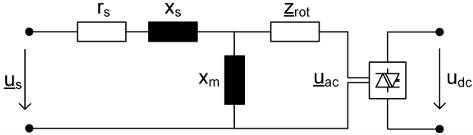
\includegraphics[width=0.75\textwidth]{contents/chapter-2/DFIG_ekivalen_PWM}
  \caption[Rangkaian Ekivalen DFIG dengan Konverter RSC Terintegrasi]{Rangkaian
  Ekivalen DFIG dengan Konverter RSC Terintegrasi \cite{digsilent2024doubly}}
  \label{fig:dfig_equiv_pwm}
\end{figure}

Sudut kerangka referensi sinkron $\phi_m$ menentukan orientasi vektor tegangan rotor
relatif terhadap kerangka stasioner jaringan dan berevolusi sesuai frekuensi slip
\cite{digsilent2024doubly}:

\begin{equation}
  \frac{d\phi_m}{dt} = 2\pi\,f_{nom}\,(\mathrm{speed} - f_{ref})
  \label{eq:dfig-phim-pf}
\end{equation}

dengan \textit{speed} adalah kecepatan rotor per unit dan $f_{ref}$ adalah frekuensi
referensi mesin acuan sistem. Transformasi antara kerangka jaringan dan kerangka rotor
\cite{digsilent2024doubly}:

\begin{align}
  i_{rd} + j\,i_{rq} &= \underline{i}_R\,e^{-j\phi_m}
  \label{eq:dfig-dq-i} \\[4pt]
  u_{rd} + j\,u_{rq} &= (u_{sr} + j\,u_{si})\,e^{-j\phi_m}
  \label{eq:dfig-dq-u}
\end{align}

Pada konfigurasi DFIG dengan konverter RSC terintegrasi, indeks modulasi PWM
$P_{md} + j\,P_{mq}$ dikonversi ke kerangka jaringan melalui \cite{digsilent2024doubly}:

\begin{equation}
  P_{mr} + j\,P_{mi} = (P_{md} + j\,P_{mq})\,e^{j\phi_m}
  \label{eq:dfig-pwm}
\end{equation}

dan tegangan rotor aktual dihitung dari indeks modulasi dan tegangan DC bus:

\begin{equation}
  u_{sr} = \frac{\sqrt{3}}{2\sqrt{2}}\,P_{mr}\,u_{dc}
    \cdot \frac{u_{dc,nom}}{U_{rot}/1000}
  \label{eq:dfig-usr}
\end{equation}

\subsubsection{Variabel Keadaan DFIG dalam PowerFactory}

Variabel keadaan model stabilitas RMS DFIG dalam PowerFactory adalah sebagai berikut
\cite{digsilent2024doubly}:

\begin{equation}
  \mathbf{x}_{DFIG,PF} =
  \begin{bmatrix}\phi_m & \mathrm{speed} &
    \psi_{A1,r} & \psi_{A1,i} &
    \psi_{A2,r} & \psi_{A2,i} &
    \psi_{B,r}  & \psi_{B,i}
  \end{bmatrix}^\top
  \label{eq:dfig-pf-statevec}
\end{equation}

dengan $\phi_m$ adalah sudut kerangka referensi sinkron; $\mathrm{speed}$ adalah
kecepatan rotor per unit; $\psi_{A1,r}$ dan $\psi_{A1,i}$ adalah komponen riil dan
imajiner fluks sangkar luar (A1); $\psi_{A2,r}$ dan $\psi_{A2,i}$ adalah komponen
fluks sangkar dalam (A2) untuk model \textit{double cage}; $\psi_{B,r}$ dan $\psi_{B,i}$
adalah komponen fluks loop ketiga untuk model \textit{double cage with current
displacement}. Pada model \textit{single cage}, hanya $\phi_m$, $\mathrm{speed}$,
$\psi_{A1,r}$, dan $\psi_{A1,i}$ yang aktif.

Vektor keadaan $\mathbf{x}_{DFIG,PF}$~\eqref{eq:dfig-pf-statevec} bersesuaian
dengan vektor model akademik~\eqref{eq:dfig-statevec} melalui pemetaan:
$\phi_m$ bersesuaian dengan sudut referensi osilasi stator, $\mathrm{speed}$
bersesuaian dengan $\omega_r$, dan komponen fluks $\psi_{A1}$ bersesuaian dengan
$\Psi_{qr} + j\Psi_{dr}$ dalam kerangka dq.

\subsubsection{Struktur Model Komposit Template DFIG WTG}

Template \textit{DIgSILENT DFIG WTG 2.5MW} mengorganisasi model dalam
\textit{composite model} "DFIG Control" dengan definisi \textit{frame}
\textit{Generic DFIG-Turbine\_resync} \cite{digsilent2024dfig}. Slot-slot utama
beserta fungsinya dirangkum pada Tabel~\ref{tab:dfig-template-slots}.

\begin{table}[H]
\centering
\caption[Slot Model Komposit DFIG Control pada Template DIgSILENT DFIG WTG 2.5MW]{Slot Model Komposit DFIG Control pada Template DIgSILENT DFIG WTG 2.5MW
\cite{digsilent2024dfig}}
\label{tab:dfig-template-slots}
\small
\begin{tabular}{p{3.8cm} p{1.6cm} p{7.8cm}}
\toprule
\textbf{Slot} & \textbf{Tipe} & \textbf{Fungsi} \\
\midrule
\texttt{DFIG} & \texttt{ElmAsm} & Mesin induksi dikonfigurasi sebagai DFIG \\
\texttt{Compensation} & DSL & Transformasi koordinat tegangan rotor \\
\texttt{Current Measurement} & DSL & Menghitung arus rotor dari sudut dan $i_d/i_q$ \\
\texttt{Ir-ctrl} & DSL & Menghitung tegangan referensi rotor dari setpoint arus \\
\texttt{PQ Control} & DSL & Mengatur daya aktif dan reaktif melalui arus rotor \\
\texttt{Speed-Ctrl} & DSL & Menghitung referensi daya dari kecepatan rotor \\
\texttt{MPT} & DSL & Pelacak daya maksimum; menghitung kecepatan optimal \\
\texttt{Turbine} & DSL & Menghitung daya angin dari sudut pitch, kecepatan, dan angin \\
\texttt{Shaft} & DSL & Menghitung daya mekanik dan kecepatan rotor \\
\texttt{Pitch Control} & DSL & Mengontrol sudut pitch sudu di atas kecepatan nominal \\
\texttt{Protection} & DSL & Mekanisme \textit{crowbar} dan proteksi kecepatan/tegangan \\
\texttt{SlowFrequMeas} & \texttt{ElmPhi} & PLL frekuensi lambat untuk pengukuran frekuensi \\
\texttt{Theta meas.} & \texttt{ElmPhi} & PLL cepat untuk pengukuran sudut tegangan \\
\bottomrule
\end{tabular}
\end{table}

Hierarki kontrol beroperasi dari luar ke dalam: \texttt{MPT} menghasilkan referensi
kecepatan optimal dari karakteristik daya angin, \texttt{Speed-Ctrl} mengonversinya
menjadi referensi daya aktif, \texttt{PQ Control} menerjemahkan referensi daya ke
setpoint arus rotor $i_{qr}^*$ dan $i_{dr}^*$, dan \texttt{Ir-ctrl} menghitung
tegangan rotor yang diperintahkan ke RSC.

Mekanisme \textit{crowbar} pada slot \texttt{Protection} diaktifkan ketika arus rotor
melebihi ambang \textit{Maxirotor} $= 2{,}0$~p.u.\ untuk melindungi konverter RSC dari
arus lebih \cite{digsilent2024dfig}. Saat \textit{crowbar} aktif, induktansi tambahan
disisipkan ke rangkaian rotor dan DFIG dapat terlepas dari busbar. Parameter proteksi
standar ditabulasikan pada Tabel~\ref{tab:dfig-protection}.

\begin{table}[H]
\centering
\caption[Parameter Blok Proteksi DFIG pada Template DIgSILENT DFIG WTG 2.5MW]{Parameter Blok Proteksi DFIG pada Template DIgSILENT DFIG WTG 2.5MW
\cite{digsilent2024dfig}}
\label{tab:dfig-protection}
\small
\begin{tabular}{p{3.2cm} p{8.2cm} p{1.2cm} p{1.0cm}}
\toprule
\textbf{Parameter} & \textbf{Deskripsi} & \textbf{Nilai} & \textbf{Sat.} \\
\midrule
\texttt{Maxirotor}   & Arus rotor untuk aktivasi \textit{crowbar} & 2{,}0 & p.u. \\
\texttt{tbypass}     & Waktu penyisipan \textit{crowbar}           & 0{,}06 & s \\
\texttt{MaxSpeed1}   & Batas kecepatan lebih tahap 1               & 1{,}5 & p.u. \\
\texttt{MaxSpeed2}   & Batas kecepatan lebih tahap 2               & 1{,}4 & p.u. \\
\texttt{MinSpeed1}   & Batas kecepatan kurang tahap 1              & 0{,}6 & p.u. \\
\texttt{MaxVoltage1} & Batas tegangan lebih tahap 1                & 1{,}5 & p.u. \\
\texttt{MinVoltage1} & Batas tegangan kurang tahap 1               & 0{,}2 & p.u. \\
\texttt{Usynch}      & Tegangan minimum untuk resinkronisasi       & 0{,}9 & p.u. \\
\bottomrule
\end{tabular}
\end{table}

\subsection{Pemodelan PMSG-WT}

PMSG-WT (\textit{Permanent Magnet Synchronous Generator Wind Turbine}, Tipe 4)
merupakan teknologi turbin angin \textit{full-rated converter} di mana seluruh daya
terkalibrasi mengalir melalui rangkaian konverter dua tahap sebelum disuntikkan ke
jaringan. Topologi sistem PMSG-WT, sebagaimana ditunjukkan pada Gambar
\ref{fig:pmsg_model}, terdiri dari lima subsistem utama yang terhubung secara
seri: PMSG yang mengubah energi mekanik rotor turbin menjadi energi listrik tiga
fasa, \textit{Rotor-Side Converter} (RSC) yang berperan sebagai penyearah AC/DC
terkontrol, tautan DC (\textit{DC link}) dengan kapasitor penyangga yang
mempertahankan tegangan $V_{DC}$, \textit{Grid-Side Converter} (GSC) yang berperan
sebagai inverter DC/AC terkontrol, serta transformator penaik tegangan untuk
interkoneksi ke jaringan transmisi \cite{dampingtorquepmsg}. RSC dan GSC masing-masing
dikendalikan oleh \textit{RSC controller} dan \textit{GSC controller} yang beroperasi
secara independen dengan tujuan kontrol yang berbeda.

\begin{figure}[H]
  \centering
  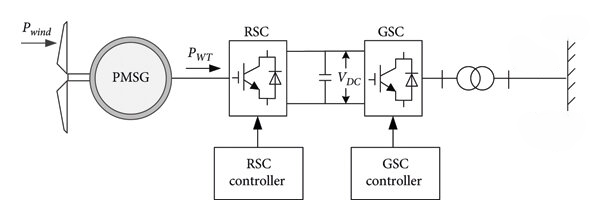
\includegraphics[width=0.85\textwidth]{contents/chapter-2/PMSGModel}
  \caption[Topologi Sistem PMSG-WT]{Topologi Sistem PMSG-WT \cite{dampingtorquepmsg}}
  \label{fig:pmsg_model}
\end{figure}

Keunggulan fundamental topologi ini terletak pada pemisahan elektris penuh
(\textit{full electrical decoupling}) antara dinamika PMSG dan dinamika jaringan.
Pada DFIG-WT, stator terhubung langsung ke jaringan sehingga \textit{flux linkage}
stator berpartisipasi dalam \textit{electromechanical oscillation mode} sistem; pada
PMSG-WT, seluruh pertukaran energi dengan jaringan AC dimediasi oleh GSC yang
bertindak sebagai antarmuka terkontrol. Akibatnya, dari perspektif jaringan, PMSG-WT
berperilaku ekivalen sebagai sumber arus terkontrol yang karakteristik dinamisnya
ditentukan sepenuhnya oleh bandwidth loop kontrol konverter, bukan oleh konstanta
elektromagnetik PMSG itu sendiri \cite{knuppel2009small}.

Dinamika listrik PMSG dimodelkan dalam kerangka referensi $dq$ sinkron yang berputar
dengan kecepatan rotor $\omega_r$. Persamaan tegangan sumbu $d$ dan $q$ mengikuti
hukum tegangan Kirchhoff dengan memperhitungkan suku kopling silang (\textit{cross-coupling})
akibat rotasi kerangka referensi \cite{wu2009small}:

\begin{align}
  L_d \frac{dI_d}{dt} &= V_d - R_s I_d + \omega_r L_q I_q
  \label{eq:pmsg-Id} \\[4pt]
  L_q \frac{dI_q}{dt} &= V_q - R_s I_q - \omega_r (L_d I_d + \lambda_f)
  \label{eq:pmsg-Iq}
\end{align}

Rangkaian ekivalen PMSG sumbu $d$ dan sumbu $q$ dalam kerangka referensi sinkron
ditunjukkan pada Gambar~\ref{fig:pmsg_daxis} dan Gambar~\ref{fig:pmsg_qaxis}
\cite{rolan2009modeling}.

\begin{figure}[H]
  \centering
  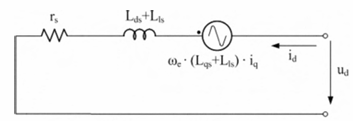
\includegraphics[width=0.75\textwidth]{contents/chapter-2/PMSG_daxis}
  \caption[\textit{D-Axis Equivalent Circuit} PMSG dalam Kerangka Referensi Sinkron]
  {\textit{D-Axis Equivalent Circuit} PMSG dalam Kerangka Referensi Sinkron
  \cite{rolan2009modeling}}
  \label{fig:pmsg_daxis}
\end{figure}

\begin{figure}[H]
  \centering
  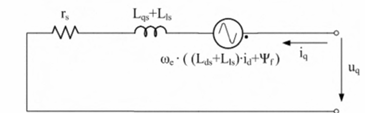
\includegraphics[width=0.75\textwidth]{contents/chapter-2/PMSG_qaxis}
  \caption[\textit{Q-Axis Equivalent Circuit} PMSG dalam Kerangka Referensi Sinkron]
  {\textit{Q-Axis Equivalent Circuit} PMSG dalam Kerangka Referensi Sinkron
  \cite{rolan2009modeling}}
  \label{fig:pmsg_qaxis}
\end{figure}

dengan $L_d$ dan $L_q$ adalah induktansi sumbu $d$ dan $q$, $R_s$ adalah resistansi
stator, $V_d$ dan $V_q$ adalah tegangan terminal sumbu $d$ dan $q$, serta $\lambda_f$
adalah \textit{flux linkage} magnet permanen. Suku $\omega_r L_q I_q$ pada persamaan
sumbu $d$ dan suku $\omega_r L_d I_d$ pada persamaan sumbu $q$ merupakan gaya gerak
listrik (\textit{back-EMF}) akibat kopling silang yang wajib dikompensasi oleh RSC
controller untuk memperoleh respons arus yang terpisah (\textit{decoupled}).

Torsi elektromagnetik yang dibangkitkan PMSG merupakan superposisi kontribusi
komponen magnet permanen dan reaksi jangkar diferensial \cite{wu2009small}:

\begin{equation}
  T_e = \frac{3}{2}\,p\,\bigl[\lambda_f I_q + (L_d - L_q)\,I_d I_q\bigr]
  \label{eq:pmsg-Te}
\end{equation}

dengan $p$ adalah jumlah pasang kutub. Suku pertama $\lambda_f I_q$ merupakan torsi
magnet permanen yang proporsional terhadap arus sumbu $q$, sedangkan suku kedua
$(L_d - L_q)I_d I_q$ adalah torsi reluktansi yang bernilai nol pada mesin PMSG
nonsalient di mana $L_d = L_q$. Dalam strategi \textit{Maximum Torque per Ampere}
(MTPA), RSC controller umumnya menerapkan referensi $I_d^* = 0$ pada PMSG nonsalient
sehingga torsi dikontrol eksklusif melalui $I_q$.

Dinamika mekanik rotor turbin-generator dinyatakan oleh persamaan ayunan massa
tunggal:

\begin{equation}
  \frac{2H_r}{\omega_s}\frac{d\omega_r}{dt} = T_m - T_e
  \label{eq:pmsg-omega}
\end{equation}

dengan $H_r$ adalah konstanta inersia rotor PMSG-WT dan $T_m$ adalah torsi mekanik
masukan dari sudu turbin. Kecepatan $\omega_r$ pada PMSG-WT bebas bervariasi sesuai kecepatan angin karena
RSC memisahkan frekuensi generator dari frekuensi jaringan.

Tautan DC yang menghubungkan RSC dan GSC berfungsi sebagai penyangga energi antar
kedua konverter. Dinamika tegangan tautan DC $V_{dc}$ mengikuti persamaan
keseimbangan daya pada kapasitor:

\begin{equation}
  C_{dc}\frac{dV_{dc}}{dt} = I_{gen} - I_{grid}
  \label{eq:pmsg-Vdc}
\end{equation}

dengan $C_{dc}$ adalah kapasitansi tautan DC, $I_{gen}$ adalah arus ekivalen dari
sisi generator (keluaran RSC), dan $I_{grid}$ adalah arus ekivalen ke sisi jaringan
(masukan GSC). Regulasi $V_{dc}$ pada nilai referensi merupakan fungsi utama GSC
controller yang dilaksanakan melalui pengaturan komponen arus sumbu $d$ pada titik
sambung jaringan.

RSC controller menjalankan kontrol orientasi fluks (\textit{field-oriented control},
FOC) dengan sumbu $q$ sejajar dengan vektor \textit{flux linkage} magnet permanen.
Referensi kecepatan optimal $\omega_r^*$ diturunkan dari karakteristik daya optimal
turbin \cite{wu2009small}:

\begin{equation}
  P_{opt} = k_{opt}\,\omega_r^3
  \label{eq:pmsg-mppt}
\end{equation}

dengan $k_{opt}$ adalah konstanta yang bergantung pada geometri turbin, kerapatan
udara, dan koefisien daya optimal $C_{p,\max}$. Loop kontrol kecepatan RSC
menghasilkan referensi torsi, yang kemudian diterjemahkan menjadi referensi arus
sumbu $q$ ($I_{qr}^*$) sesuai hubungan $T_e^* = \frac{3}{2}p\lambda_f I_{qr}^*$.
Kompensasi kopling silang diterapkan untuk mengisolasi dinamika loop $d$ dan $q$,
sehingga bandwidth kontrol arus dapat dioptimalkan secara independen.

GSC controller menjalankan kontrol vektor arus (\textit{current vector control})
dalam kerangka referensi sinkron yang terkunci ke tegangan titik sambung melalui
\textit{Phase-Locked Loop} (PLL). Regulasi komponen arus sumbu $d$ jaringan
mengendalikan pertukaran daya reaktif (atau tegangan titik sambung), sedangkan
regulasi komponen arus sumbu $q$ jaringan mengendalikan injeksi daya aktif sekaligus
menjaga keseimbangan $V_{dc}$. Pemisahan kontrol daya aktif dan reaktif yang
dihasilkan oleh kerangka referensi tegangan-sinkron ini memungkinkan PMSG-WT
memenuhi persyaratan \textit{grid code} terkait kapabilitas daya reaktif secara
dinamis \cite{wu2009small}.

Variabel keadaan model linearisasi PMSG-WT tersusun dalam vektor:

\begin{equation}
  \mathbf{x}_{PMSG} =
  \begin{bmatrix}I_d & I_q & \omega_r & V_{dc}\end{bmatrix}^\top
  \label{eq:pmsg-statevec}
\end{equation}

ditambah variabel keadaan internal kontroler RSC dan GSC (integrator PI, keadaan PLL).
Karena konverter penuh memisahkan PMSG dari jaringan, variabel keadaan sisi
generator ($I_d$, $I_q$, $\omega_r$) tidak berpartisipasi langsung dalam
\textit{electromechanical oscillation mode} sistem dan tidak akan muncul sebagai
kontributor dominan dalam analisis \textit{participation factor} pada \textit{electromechanical mode} \cite{knuppel2009small}. Kontribusi PMSG-WT terhadap kestabilan
sinyal kecil sistem pada umumnya dimediasi melalui dinamika PLL dan loop kontrol
tegangan GSC, yang dapat berinteraksi dengan \textit{electromechanical mode} sistem dalam kondisi
tertentu \cite{li2024smallsignal}. Dalam penelitian ini, model PMSG-WT menggunakan
\textit{template} bawaan DIgSILENT PowerFactory 2024 \cite{digsilent2024frc} tanpa
modifikasi parameter kontrol.

\subsubsection{Model PowerFactory: Static Generator sebagai Antarmuka FRC}

Dalam DIgSILENT PowerFactory 2024, PMSG-WT dengan konverter penuh dimodelkan sebagai
\textit{Static Generator} (elemen \texttt{ElmGenstat}) \cite{digsilent2024sg}.
Template \textit{DIgSILENT FullyRatedConv WTG 2.5MW} hanya merepresentasikan
\textit{grid-side converter}; bagian mekanik rotor dan aerodinamika tidak disertakan
\cite{digsilent2024frc}. Keputusan pemodelan ini dibenarkan karena konverter VSC
frekuensi memisahkan rotor dan generator dari jaringan secara penuh, sehingga dinamika
sisi generator tidak muncul dalam matriks sistem $\mathbf{A}$ pada titik operasi
jaringan.

Elemen \texttt{ElmGenstat} merepresentasikan PMSG-WT sebagai sumber arus terkontrol
pada titik sambung jaringan. Nilai arus injeksi dipasok oleh blok \textit{Current
Controller} yang menerima referensi dari \textit{PQ Control}:

\begin{equation}
  \underline{i}_{gen} = i_d + j\,i_q \quad \text{(per unit)}
  \label{eq:frc-igen}
\end{equation}

dengan komponen $i_d$ mengendalikan daya reaktif atau tegangan terminal, dan komponen
$i_q$ mengendalikan injeksi daya aktif. Pemisahan kontrol $d$-$q$ ini dimungkinkan oleh
\textit{Phase-Locked Loop} (PLL) yang mengunci sudut tegangan terminal $\theta_{PLL}$
sebagai referensi kerangka koordinat sinkron.

\subsubsection{Struktur Model Komposit dan Variabel Keadaan}

\textit{Composite model} "FullyRatedConv Control" menggunakan definisi \textit{frame
WTG FRC Frame incl Current Ctrl} \cite{digsilent2024frc}. Slot-slot utama beserta
fungsinya ditampilkan pada Tabel~\ref{tab:frc-template-slots}.

\begin{table}[H]
\centering
\caption[Slot Model Komposit \textit{FullyRatedConv Control} pada Template DIgSILENT FullyRatedConv WTG 2.5MW]{Slot Model Komposit \textit{FullyRatedConv Control} pada Template DIgSILENT
FullyRatedConv WTG 2.5MW \cite{digsilent2024frc}}
\label{tab:frc-template-slots}
\small
\setlength{\tabcolsep}{5pt}
\begin{tabular}{p{3.8cm} p{2.3cm} p{7.1cm}}
\toprule
\textbf{Slot} & \textbf{Tipe} & \textbf{Fungsi} \\
\midrule
\texttt{Generator} & \texttt{ElmGenstat} & \textit{Static generator} sebagai antarmuka jaringan \\
\texttt{Current Controller} & DSL & Menghitung sinyal tegangan referensi dari setpoint arus \\
\texttt{PQ Control} & DSL & Mengatur daya aktif dan reaktif melalui setpoint arus \\
\texttt{PLL} & \texttt{ElmPhi} & Pengukuran sudut tegangan cepat untuk sinkronisasi jaringan \\
\texttt{Slow FrequMeas} & \texttt{ElmPhi} & Pengukuran frekuensi lambat untuk reduksi daya \\
\texttt{ActivePowerReduction} & DSL & Mengurangi injeksi daya saat frekuensi jaringan melebihi batas \\
\bottomrule
\end{tabular}
\end{table}

Variabel keadaan gabungan model FRC-WTG dalam simulasi RMS mencakup:

\begin{equation}
  \mathbf{x}_{FRC,PF} =
  \begin{bmatrix}\theta_{PLL} & i_d & i_q\end{bmatrix}^\top
  \label{eq:frc-pf-statevec}
\end{equation}

ditambah variabel keadaan integrator PI pada loop arus \texttt{Current Controller} dan
integrator \texttt{PQ Control}. Sudut $\theta_{PLL}$ adalah satu-satunya variabel
keadaan yang mengkopelkan FRC-WTG dengan dinamika tegangan jaringan secara langsung.
Arus $i_d$ dan $i_q$ mengikuti referensi melalui bandwidth \textit{inner current control
loop} (10--50~ms), terlalu cepat untuk berinteraksi dengan
\textit{electromechanical oscillation mode} (0{,}1--2{,}0~Hz); FRC-WTG tidak
berpartisipasi langsung dalam \textit{electromechanical oscillation mode}
sistem \cite{knuppel2009small}.

\subsubsection{Dukungan Daya Reaktif dan Karakteristik \textit{Grid Code}}

Template FRC-WTG mengimplementasikan dukungan tegangan saat gangguan sesuai
Transmission Code 2007 Jerman dan SDLWindV \cite{digsilent2024frc}. Ketika tegangan
terminal turun melewati \textit{deadband} $\Delta U_{min}$, \textit{PQ Controller}
meningkatkan injeksi arus reaktif secara proporsional:

\begin{equation}
  \Delta i_q = K \cdot \Delta U, \qquad \Delta U = U_{ref} - U_{terminal}
  \label{eq:frc-qsupport}
\end{equation}

dengan $K$ adalah penguatan arus reaktif yang dapat dikonfigurasi. Kemampuan injeksi
arus reaktif hingga 1{,}0~p.u.\ dalam rentang waktu milidetik menjadikan FRC-WTG
lebih unggul dari DFIG-WT dalam mendukung profil tegangan jaringan pasca-gangguan,
karena DFIG-WT dibatasi oleh kapasitas konverter \textit{partial-rated}.


\subsection{Sistem Uji IEEE \textit{Nine-Bus}}

Sistem uji dalam penelitian ini adalah sistem IEEE \textit{nine-bus} yang dikembangkan
oleh Anderson dan Fouad \cite{anderson1977power}. Sistem ini merupakan \textit{benchmark}
standar yang paling banyak digunakan dalam penelitian kestabilan sistem tenaga, dengan
\textit{electromechanical} parameter terdokumentasi secara lengkap dan topologi meshing tiga-mesin
yang merepresentasikan karakteristik fundamental jaringan transmisi skala nyata.
Sistem beroperasi pada frekuensi 60~Hz dengan tegangan dasar 230~kV pada sisi transmisi.

\begin{figure}[H]
  \centering
  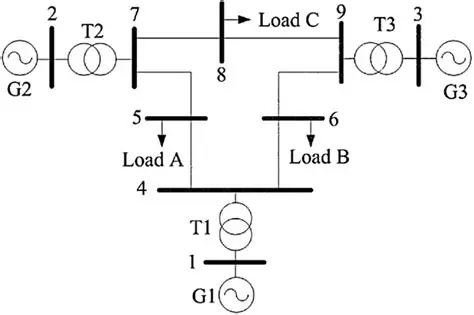
\includegraphics[width=0.72\textwidth]{contents/chapter-2/IEEE9Bus}
  \caption[Topologi Sistem Uji IEEE \textit{Nine-Bus}]{Topologi Sistem Uji IEEE
  \textit{Nine-Bus} \cite{yousefikia2023novel}}
  \label{fig:ieee9bus_ch2}
\end{figure}

Sebagaimana ditunjukkan pada Gambar~\ref{fig:ieee9bus_ch2}, sistem terdiri dari
sembilan bus yang diorganisasi dalam dua hierarki tegangan. Tiga bus generator
(bus~1, 2, dan~3) beroperasi pada tegangan pembangkitan dan terhubung ke jaringan
transmisi 230~kV melalui transformator penaik tegangan T1, T2, dan T3. Bus~1
(Generator G1, 247{,}5~MVA) berfungsi sebagai \textit{slack bus} yang menyediakan
referensi sudut dan mengkompensasi rugi-rugi transmisi secara real-time. Bus~2
(Generator G2, 192~MVA) dan bus~3 (Generator G3, 128~MVA) merupakan bus generator
berkontrol tegangan (\textit{PV bus}) dengan daya aktif yang ditentukan dari hasil
\textit{load flow}.

Jaringan transmisi 230~kV mencakup enam saluran transmisi yang membentuk topologi
\textit{meshed}: saluran 4--5, 4--6, 5--7, 6--9, 7--8, dan 8--9. Ketiga beban
terpusat tersambung pada bus~5 (Beban A, 125{,}0~MW $+$ $j$50{,}0~MVAR), bus~6
(Beban B, 90{,}0~MW $+$ $j$30{,}0~MVAR), dan bus~8 (Beban C, 100{,}0~MW $+$
$j$35{,}0~MVAR) \cite{anderson1977power}. Struktur \textit{ring} yang dibentuk oleh
saluran 7--8--9 dengan titik interkoneksi di bus~4, 5, dan~6 menciptakan dua jalur
aliran daya kompetitif antara G2, G3, dan pusat beban, sehingga menghasilkan profil
pertukaran daya antar-area yang representatif untuk pengujian SSS.

Parameter inersia ketiga generator adalah $H_1 = 23{,}64$~MWs/MVA (G1, bus~1),
$H_2 = 6{,}40$~MWs/MVA (G2, bus~2), dan $H_3 = 3{,}01$~MWs/MVA (G3, bus~3)
\cite{anderson1977power}. Dispersi nilai $H$ yang mencapai hampir satu dekade
($H_1/H_3 \approx 7{,}9$) merupakan faktor penentu utama distribusi energi kinetik
antar-mesin: mesin berinersia tinggi (G1) merespons gangguan dengan laju perubahan
kecepatan yang jauh lebih lambat dibandingkan mesin berinersia rendah (G3), sehingga
perbedaan fase osilasi antar-mesin berkembang secara signifikan pasca-gangguan. Efek
ini mendorong munculnya dua \textit{electromechanical oscillation mode} yang dapat
diidentifikasi secara terpisah, sesuai dengan teorema bahwa sistem $n$-mesin memiliki
tepat $(n-1)$ mode osilasi antar-mesin.

Kedua \textit{electromechanical oscillation mode} sistem ini berada pada rentang
frekuensi \textit{local mode} (0{,}8--2{,}0~Hz), mencerminkan kuatnya kopling
elektris ketiga generator dalam satu area tunggal tanpa interkoneksi antar-area yang
lemah. Mode pertama umumnya melibatkan G2 dan G3 yang berayun dengan fase berlawanan
terhadap G1, sedangkan mode kedua mencirikan pola osilasi yang berbeda antara pasangan
generator lainnya. Nilai \textit{eigenvalue}, \textit{damping ratio}, dan distribusi
\textit{participation factor} sistem ini telah terdokumentasi dengan baik dalam
literatur, menjadikannya acuan perbandingan yang valid dalam studi dampak integrasi
pembangkit berbasis konverter terhadap karakteristik modal sistem tenaga
\cite{wang2014small,he2015investigation}.

Sistem ini dipilih karena parameternya terdokumentasi baik, digunakan luas sebagai
\textit{benchmark} dalam penelitian SSS dengan penetrasi PLTB, dan tersedia sebagai
contoh bawaan di DIgSILENT PowerFactory 2024
\cite{anderson1977power,wang2014small,he2015investigation,sun2013small}.

